\documentclass[lang=cn,newtx,10pt,scheme=chinese]{elegantbook}

\title{计算机系统课程设计(编译器)指导手册}
\subtitle{ACM班}

\author{}
\institute{ACM班编译器助教组}
\date{2023/07/02}
\version{0.8.0}
% \bioinfo{自定义}{信息}

% \extrainfo{注意:本模板自 2023 年 1 月 1 日开始,不再更新和维护!}

\setcounter{tocdepth}{3}

% \logo{logo-blue.png}
\cover{cover.jpg}



% 本文档命令
\usepackage{array}
\newcommand{\ccr}[1]{\makecell{{\color{#1}\rule{1cm}{1cm}}}}

% 修改标题页的橙色带
\definecolor{customcolor}{RGB}{32,178,170}
\colorlet{coverlinecolor}{customcolor}
\usepackage{cprotect}

\addbibresource[location=local]{reference.bib} % 参考文献,不要删除

\begin{document}

\maketitle

\frontmatter

\tableofcontents

\mainmatter

\chapter{课程要求}
% \begin{introduction}
%     \item TBA
% \end{introduction}

编译器设计课程在 ACM 班有非常悠久的历史,该课程要求学生自主完成一个从源代码到汇编代码的编译器,引导学生直观理解系统执行二进制代码的过程并掌握一系列代码级别优化方法。
与传统编译原理课程不同的是,本课程不会提供任何的已有框架。课程设计目标要求自主设计数据结构(自主设计抽象语法树、中间表达,自主探索语言特定的优化策略)。

\begin{remark}
  \begin{enumerate}
    \item 在本课程中,允许使用 \texttt{antlr} 等前端分析库,但是不得使用现有的编译库。
    \item 作业仓库:\url{https://github.com/ACMClassCourses/Compiler-Design-Implementation}。其中 testcases 目录下提供了不同阶段的评测点,
      每个阶段的目录下提供了测试脚本,脚本中的注释提供了用法提示。
    \item 运行环境(模拟器):\url{https://github.com/Engineev/ravel}。
  \end{enumerate}
\end{remark}

\section{为什么需要编译器?}

程序设计中,我们总是会将语言区分为低级语言 (low-level programming language) 与
高级语言 (high-level programming language)。

低级语言一般鲜有对体系结构的抽象,总是与硬件相耦合。正因如此,低级语言难以移植到其他的硬件平台,
但优势在于可以不借助任何复杂的工具(如编译器)而直接转化为机器码。

高级语言会将操作进行高度抽象,形成一种人类可读且易于移植的语言。因此,相较于低级语言,
高级语言的编写效率是非常高的。这也是我们平时接触的绝大多数语言都是高级语言的原因。然而,正是因为这样的抽象,
其无法很方便地转化到机器码。

假设我们有一段 C 语言编写的 hello world 的程序 hello\_world.c,如果我们想要在机器上运行这段程序,
其需要经历以下阶段:
\begin{enumerate}
  \item 由 C 的预处理器 (\textbf{C} \textbf{p}re\textbf{p}rocesser, cpp)
    将所有宏展开(如 \texttt{\#include} 宏会将对应的文件拷贝过来),生成预处理后的文件(如 hello\_world.i)。
  \item 由编译器将预处理后的结果转化为汇编 (assembly)(如 hello\_world.s)。
  \item 由汇编器将汇编转化为目标代码 (object code)(如 hello\_world.o)。
  \item 由链接器将若干份目标代码链接为可执行文件。此阶段中,会处理不同翻译单元中的互相引用变量及函数。
  \item 由操作系统动态链接需要的依赖库后运行程序。
\end{enumerate}

可以看到,一个编译器实际上是将预处理后的代码转化为汇编的工具。不过,我们平时接触的编译器同时集成了预处理器、汇编器、链接器,
因此我们在使用时会省略一部分阶段。

\section{编译器具体阶段}

以下是实现编译器的步骤的概述:

\begin{enumerate}
    \item 词法分析:第一步是将源代码转换为一个词素流,在这个阶段需要指定基本的词素单元。
    \item 句法分析:根据生成的词素流分析源代码的结构并且按照语言的语法规则转换为层次化的结构,生成解析树或抽象语法树(AST)。
    \item 语义分析:解析后,进行语义分析以检查程序的正确性。这包括类型检查、名称解析、作用域分析和其他语义检查。在这个阶段需要构建一个符号表并执行各种检查,以确保程序的正确性。
    \item 中间表示:在这个阶段,将AST转换为中间表示 (IR)。IR是程序的一个抽象表示,更容易分析和优化。常见的 IR 大多使用虚拟寄存器的抽象。
    \item 代码优化:根据生成的中间表示对程序进行优化,其中关键一步是分配寄存器(如果采用虚拟寄存器抽象需要转换为真实的寄存器)。此外,优化还包括死代码消除、函数内联等。
    \item 代码生成:优化后,生成目标汇编代码。该步骤需要将源语言/中间表达映射到目标体系结构的相应汇编指令,需要指令选择,以生成高效的汇编代码。
\end{enumerate}

\section{编译器作业阶段及对应要求}

为了方便大家分阶段开发,我们将会把作业划分为三个阶段。语义检查阶段(对应1、2、3)、目标代码生成阶段(阶段4、6)、寄存器分配(阶段5)。各个阶段的要求如下:
\begin{table}[!ht]
    \resizebox{\textwidth}{!}{\begin{tabular}{c|c|c}
        \hline
                 & 目标                                                                          & 要求                                                                            \\ \hline
        语义检查阶段   & \begin{tabular}[c]{@{}c@{}}将源代码转换为一个具有语义信息的\\ 抽象结构并实现对语言的语法检查。\end{tabular} & \begin{tabular}[c]{@{}c@{}}通过编译器可以识别存在语法错\\ 误的代码。\end{tabular}                \\ \hline
        目标代码生成阶段 & \begin{tabular}[c]{@{}c@{}}将高级语言转换为汇编语言并且实现\\ 简单的指令选择。\end{tabular}         & \begin{tabular}[c]{@{}c@{}}可以生成对应的可终止汇编代码\\ (不对性能做出要求)。\end{tabular}          \\ \hline
        寄存器分配    & \begin{tabular}[c]{@{}c@{}}在目标代码或中间表达等结构的基础\\ 上实现高效的寄存器分配算法。\end{tabular}   & \begin{tabular}[c]{@{}c@{}}在测评程序集上与标准Clang编译的\\ 结果进行性能比对(按照周期数)。\end{tabular} \\ \hline
        \end{tabular}}
\end{table}


\chapter{语义检查}

\chapter{目标代码生成}

前面的章节中,我们已经建构了抽象语法树 (AST),并进行了类型检查。在此基础上,我们需要通过抽象语法树生成目标代码。

尽管我们的确可以从抽象语法树直接生成目标平台的代码,然而现实情况并非如此。假设我们有
$m$ 门语言,$n$ 个目标平台,那么如果采用直接生成代码,则需要写 $m\times n$
个转换程序,这对于现代编译器来说是无法承受的。但是如果我们选取一门中间语言作为转换的中转,那么我只要实现
$m$ 个从语言到中间语言的转换程序,以及 $n$ 个从中间语言到目标平台的转换程序,就可以满足需求。这样的中间语言被称为
IR (intermediate representation)。此外,对于后续的优化,也可以在 IR 上处理,这可以大大减少编译器优化工作。

本章中,我们以 LLVM Language (version 15) 为例,来展示如何从中间语言转换成目标代码。如需查看
LLVM 的完整文档,请访问 \url{https://llvm.org/docs/LangRef.html}。

\section{LLVM 15 概览}

LLVM 是一套编译器基础设施项目,包含一系列模块化的编译器组件和工具链,用来开发编译器前端和后端。

IR 是区分前后端的标志。语法检查、建构抽象语法树、生成 IR 都属于前端部分。通过 IR
生成目标代码、针对 IR 层面的优化都属于后端部分。

LLVM 提供的工具链可以检查 IR 问题、运行及调试 IR,因此我们推荐使用 LLVM IR
作为我们编译器的 IR。

LLVM 项目中有很多非常使用的工具——如 clang、llc、lli 等等。一般来是,最常用的工具是
clang,因为 clang 可以将代码编译到 LLVM IR,也可以将 LLVM 代码编译到目标平台。比如
\texttt{clang main.c -S -emit-llvm --target=riscv32-unknown-elf -o main.ll}
可以将 \texttt{main.c} 转换成 LLVM IR 并保存在 \texttt{main.ll} 中;而
\texttt{clang -S main.ll --target=riscv32-unknown-elf -o main.s}
可以将 \texttt{main.ll} 转换成汇编。llc 可以将 LLVM IR 转换成汇编,如
\texttt{llc -march=riscv32 main.ll -o main.s} 会将 \texttt{main.ll}
转换成汇编并存到 \texttt{main.s}。

LLVM IR 语言与高级语言不同,不存在多层嵌套的环境,指令以基础块 (basic block)
的形式组织,与汇编语言非常相近,同时又保留了高级语言的类型属性。选择 LLVM 15
的原因是从 LLVM 15 开始,LLVM IR 默认使用不透明指针
(Opaque Pointers),大大减少了转换时的负担。具体请参见章节 \ref{LLVM-semantic}。

LLVM IR 的一大特性是静态单赋值 (Static Single Assignment,
SSA),即变量能且仅能被赋值一次,这一特性可以让编译器的静态分析更方便。

当然,你也可以使用其他 IR 或是直接一步从 AST
转换成目标代码(因为我们的编译器只有一个目标平台)。

\section{LLVM 15 环境}

\subsection{在线 LLVM 环境}\label{online-LLVM-env}

在学习 LLVM 的过程中,一个方便的使用环境非常重要。Godbolt (
\url{https://godbolt.org/}) 提供了几乎所有的编译器,并且可以编译到大量平台。

\begin{figure}[htb]
\centering
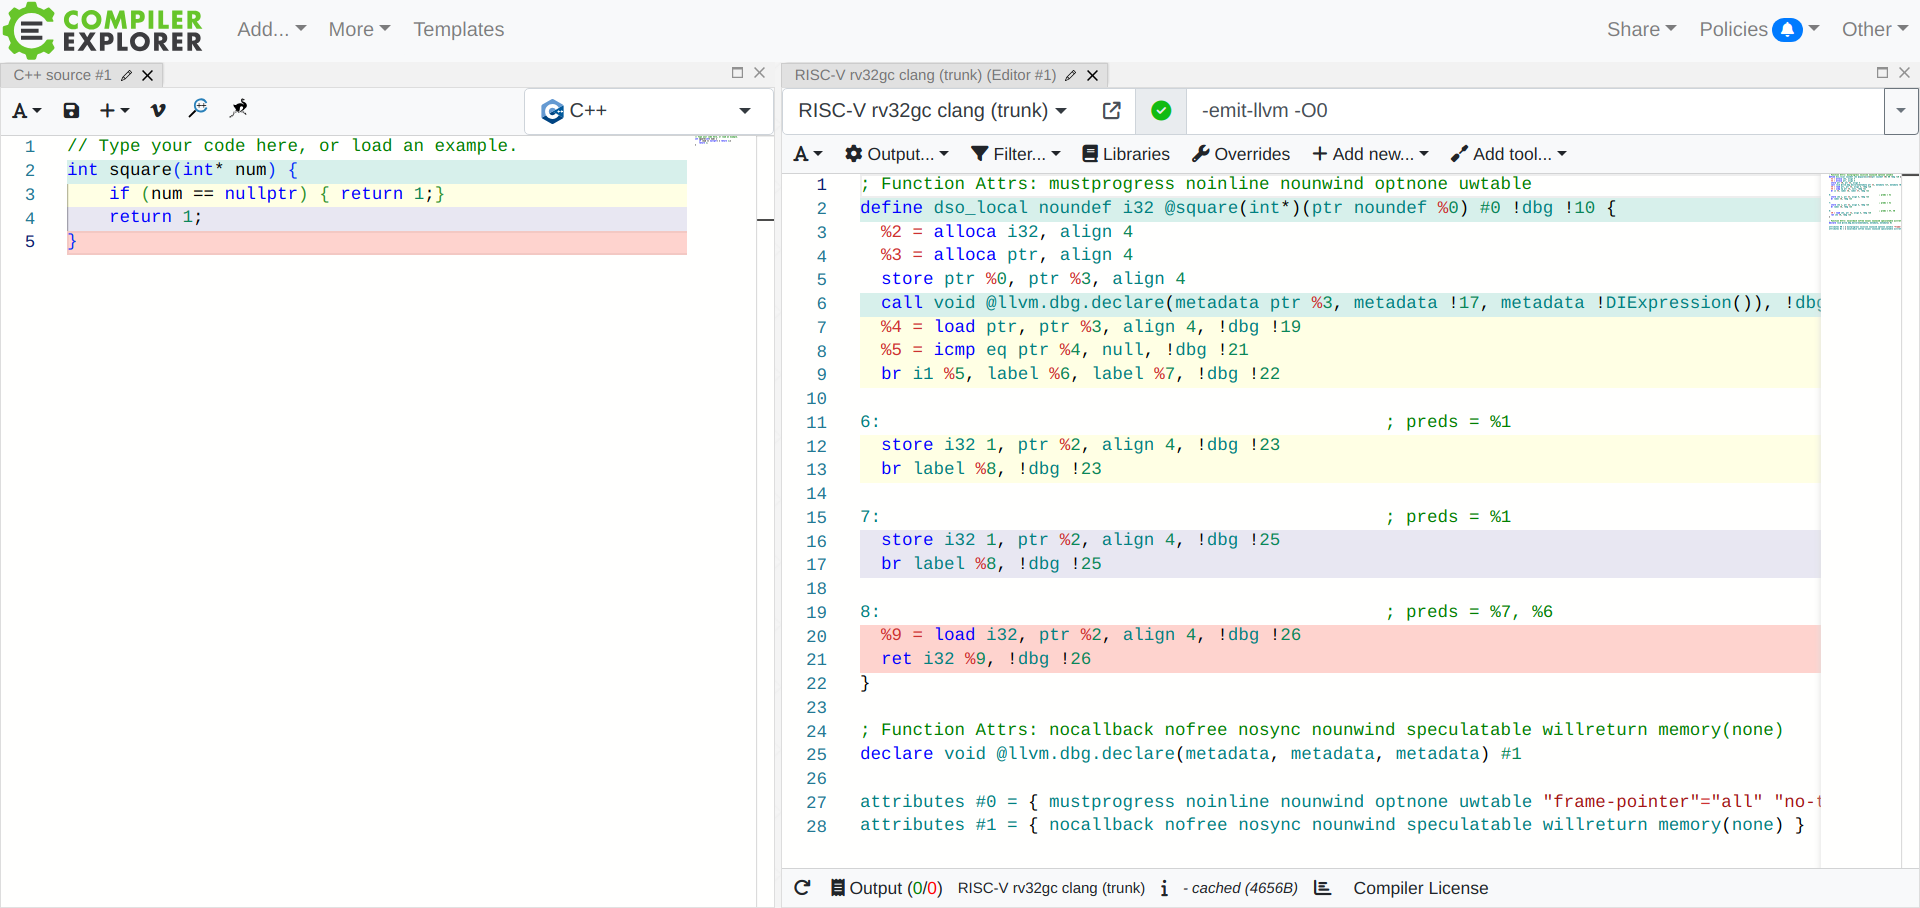
\includegraphics[scale=0.3]{image/godbolt.png}
\caption{Godbolt 使用截图}
\label{godbolt_sreenshot}
\end{figure}

图片 \ref{godbolt_sreenshot} 是一个通过在线 LLVM 环境来了解 LLVM 语言的例子。在
gofbolt 上,页面被分为两栏——左栏是你的输入,右栏是你选择的编译器在你填入的参数下的输入。下面我们将会分别介绍左右栏的使用。

左栏有一个语言选择框(位于左栏的上部)和一个代码输入框。语言选择框可以选择所使用的编程语言。

右栏上部左边部分是编译器选择框,右边部分是编译器参数框。我们此时希望将代码编译到适用于 rv32gc
平台的 LLVM 语言,而且不希望编译器做出优化(否则可能会把一部分代码直接去掉)。由于我们的编译器的目标平台是
rv32gc,且 clang 可以通过 \texttt{-emit-llvm} 来输出 LLVM 语言,因此我们在编译器选择框选择
RISCV rv32gc clang (trunk)(trunk 这里表示最新的 clang),在编译器参数框中输入 \texttt{-emit-llvm -O0}。

关于语言特性的内容,请见章节 \ref{LLVM-semantic}。

\subsection{本地 LLVM 环境}

你可以安装 LLVM 15 及其以上版本。截止 LLVM 17,所有的 LLVM 15 特性均可使用。

对于使用 apt 包管理的用户(debian/Ubuntu/... 用户),请参考 \href{https://apt.llvm.org/}{LLVM apt 安装文档}。

对于使用 pacman 包管理的用户,可以执行 \texttt{sudo pacman -S llvm clang} 安装最新版本的 LLVM。

\textit{注意:如果你用的是特定版本的 LLVM(而非最新版本),在使用程序时,需要加上} \texttt{-<version>} \textit{后缀。比如} \texttt{clang-15 ...} \texttt{。}

你可以执行 \texttt{clang --version} 来检查 clang 是否确实安装到系统中。正常情况下,该指令会显示你的
clang 版本、目标平台等信息。

\section{LLVM 15 语法}\label{LLVM-semantic}

\textit{本章节只介绍常用的 LLVM 15 语法。如需了解全部语法或更详细的 LLVM 语法,请访问
\url{https://llvm.org/docs/LangRef.html}。}

\textit{提示:你可以先大致了解 LLVM 15 语法,然后跳到「从抽象语法树到中间语言」章节
(\ref{AST-to-IR}) 了解如何完成抽象语法树到 IR
的转换。在阅读「从抽象语法树到中间语言」部分的过程中,如果对 LLVM IR
的语法有疑惑,再回到本部分查看详细信息。}

\subsection{LLVM 15 简单例子}

对于下面的代码,

\begin{lstlisting}[language=C]
int c;
int foo(int* a, int b) {
    if (a == 0) return 0;
    return  *a + b + c;
}
\end{lstlisting}

在 \texttt{-emit-llvm -O1 -fno-discard-value-names}
参数下,会生成下面的代码(下面的代码去掉了生成代码的 attribute
部分和一些注释,这些内容我们在编译器大作业中应该用不到)

\begin{lstlisting}[language=llvm]
@c = dso_local local_unnamed_addr global i32 0, align 4, !dbg !0

define dso_local i32 @foo(ptr noundef readonly %a, i32 noundef %b) local_unnamed_addr #0 !dbg !15 {
entry:
  call void @llvm.dbg.value(metadata ptr %a, metadata !20, metadata !DIExpression()), !dbg !22
  call void @llvm.dbg.value(metadata i32 %b, metadata !21, metadata !DIExpression()), !dbg !22
  %cmp = icmp eq ptr %a, null, !dbg !23
  br i1 %cmp, label %return, label %if.end, !dbg !25

if.end:                                           ; preds = %entry
  %0 = load i32, ptr %a, align 4, !dbg !26
  %add = add nsw i32 %0, %b, !dbg !31
  %1 = load i32, ptr @c, align 4, !dbg !32
  %add1 = add nsw i32 %add, %1, !dbg !33
  br label %return, !dbg !34

return:                                           ; preds = %entry, %if.end
  %retval.0 = phi i32 [ %add1, %if.end ], [ 0, %entry ], !dbg !22
  ret i32 %retval.0, !dbg !35
}
\end{lstlisting}

进一步地,我们还可以忽略一些 debug 参数、一些无用的参数(如
\texttt{dso\_local}、\texttt{local\_unnamed\_addr} 和
\texttt{align})以及不必要的 debug 函数,这样可以得到以下的代码

\begin{lstlisting}[language=llvm]
@c = global i32 0

define i32 @foo(ptr %a, i32 %b) {
entry:
  %cmp = icmp eq ptr %a, null
  br i1 %cmp, label %return, label %if.end

if.end:                       ; preds = %entry
  %0 = load i32, ptr %a
  %add = add i32 %0, %b
  %1 = load i32, ptr @c
  %add1 = add i32 %add, %1
  br label %return

return:                       ; preds = %entry, %if.end
  %retval.0 = phi i32 [ %add1, %if.end ], [ 0, %entry ]
  ret i32 %retval.0
}
\end{lstlisting}

我们会在本章每个元素一一解释。如果你设置了 \texttt{-O0},你会看到一些如
\texttt{\%3 = alloca i32} 的指令,我们也会在本章中介绍。

\subsection{LLVM 15 基本语法}

LLVM 15 的基本语法包含
\begin{itemize}
  \item 类型,如 \texttt{i1},\texttt{i32},具体参见章节 \ref{LLVM-types};
  \item 变量,如 \texttt{\@a = global i32 0} 以及
    \texttt{\%a = ...},具体参见章节 \ref{LLVM-variables};
  \item 常量,具体参见章节 \ref{LLVM-constants};
  \item 函数定义及声明,如 \texttt{define i32 \@foo(ptr \%0, i32 \%1) \{...\}},具体参见章节
    \ref{LLVM-functions};
  \item 标签 (label),如 \texttt{4:};
  \item 指令,如 \texttt{\%3 = icmp eq ptr \%0, null},具体参见章节
    \ref{LLVM-instructions}。
\end{itemize}

一个基本的 LLVM IR 翻译单元由若干类型声明、若干全局变量和若干函数定义组成。

函数定义由若干标签和若干指令组成。标签是可以被分支指令 (\ref{LLVM-br-instructions})
跳转到的地方。在函数外部的变量为全局变量,在函数内部的变量为局部变量。
所有的变量能且仅能被赋值一次(因此全局变量实际上是指向变量的指针)。

每行的分号 (\texttt{;}) 后的内容为注释。如没有注释,分号是不必要的。

\subsection{类型}\label{LLVM-types}

常用的类型有
\begin{itemize}
  \item 整数类型:用 \texttt{i<N>} 表示,如 \texttt{i32},\texttt{i1};
  \item 指针类型:用 \texttt{ptr} 表示;
  \item 数组类型:用 \texttt{[<\# elements> x <elementtype>]} 表示,如
    \texttt{[40 x i32]}。数组类型允许嵌套定义,如
    \texttt{[3 x [4 x i32]]},表示 $3\times 4$ 的二维数组。另请参见
    \url{https://llvm.org/docs/LangRef.html#array-type};
  \item 结构类型:对于普通的类,用 \texttt{\%<typename> = type \{ <type list> \}} 表示,如
    \texttt{\%mytype = type \{ \%mytype*, i32 \}};对于不能对齐的类
    (packed struct),用 \texttt{\%<typename> = type <\{ <type list> \}>}
    表示,如 \texttt{<\{ i8, i32 \}>} 表示一个 5 字节的结构体。
\end{itemize}

\subsection{变量}\label{LLVM-variables}

非匿名变量的命名必须符合 \texttt{[\%@][-a-zA-Z\$.\_][-a-zA-Z\$.\_0-9]*},且不能与作用域中的其他变量名或函数名冲突。

匿名变量的命名必须符合 \texttt{[\%@](0|[1-9][0-9]*)},且不能与作用域中的其他变量名或函数名冲突。

变量分为全局变量和局部变量。全局变量以 \texttt @ 开头,如 \texttt{@abc};局部变量以 \texttt \% 开头,如 \texttt{\%abc}。

变量能且只能被赋值一次。

\subsection{常量}\label{LLVM-constants}

常量有
\begin{itemize}
  \item boolean 常量: 仅有 \texttt{true},\texttt{false} 两个字符串,类型为 \texttt{i1}。
  \item int 常量:支持所有标准的整数。
  \item 空指针常量:仅支持字符串 \texttt{null},类型为 \texttt{ptr}。
\end{itemize}

\textit{如需使用其他常量,请参见\href{https://llvm.org/docs/LangRef.html\#constants}{官方文档}。}

\subsection{函数定义及声明}\label{LLVM-functions}

函数的定义方式如下:

\begin{lstlisting}[language=llvm]
define <ResultType> @<FunctionName>(...) { ... }
\end{lstlisting}

圆括号内为函数参数,参数用逗号分割,每项参数的形式为 \texttt{<type> [name]}。

典型的例子有:
\begin{itemize}
  \item 无入参函数 \texttt{int a()},对应的函数为 \texttt{define i32 \@a() \{...\}};
  \item 单入参函数 \texttt{void a(int x)},对应的函数为 \texttt{define void \@a(i32 \%x) \{...\}};
  \item 双入参函数 \texttt{int a(int x1, int x2)},
    对应的函数为 \texttt{define i32 \@a(i32 \%x1, i32 \%x2) \{...\}}。
\end{itemize}

花括号内为函数的指令以及若干标签 (label)。

函数的声明方式如下:

\begin{lstlisting}[language=llvm]
declare <ResultType> @<FunctionName>(...)
\end{lstlisting}

声明的形式基本上和定义一致,只不过去掉了函数体,前面的 \texttt{define} 被换成了
\texttt{declare}。

\textit{关于函数调用,请参见 call 指令 (\ref{LLVM-call-instructions})。}

\subsection{指令}\label{LLVM-instructions}

\textit{注:以下的介绍中的语法只是 LLVM IR 语法的一部分。关于全部语法,请访问
\url{https://llvm.org/docs/LangRef.html\#instruction-reference}。
同时,每个指令的章节也会附上对应的官方文档链接。}

在 LLVM IR 中,我们一般会用到以下指令:(点击括号中的章节号可以跳转到对应章节)

\begin{itemize}
  \item 二元运算指令 (\ref{LLVM-binary-instructions})
    \begin{itemize}
      \item \texttt{add} 指令
      \item \texttt{sub} 指令
      \item \texttt{mul} 指令
      \item \texttt{sdiv} 指令
      \item \texttt{srem} 指令
      \item \texttt{shl} 指令
      \item \texttt{ashr} 指令
      \item \texttt{and} 指令
      \item \texttt{or} 指令
      \item \texttt{xor} 指令
    \end{itemize}
  \item 控制流相关指令
    \begin{itemize}
      \item \texttt{br} 指令 (\ref{LLVM-br-instructions})
      \item \texttt{ret} 指令 (\ref{LLVM-ret-instructions})
    \end{itemize}
  \item 内存相关指令
    \begin{itemize}
      \item \texttt{alloca} 指令 (\ref{LLVM-alloca-instructions})
      \item \texttt{load} 指令 (\ref{LLVM-load-instructions})
      \item \texttt{store} 指令 (\ref{LLVM-store-instructions})
      \item \texttt{getelementptr} 指令 (\ref{LLVM-gep-instructions})
    \end{itemize}
  \item 其他指令
    \begin{itemize}
      \item \texttt{icmp} 指令 (\ref{LLVM-icmp-instructions})
      \item \texttt{call} 指令 (\ref{LLVM-call-instructions})
      \item \texttt{phi} 指令 (\ref{LLVM-phi-instructions})
    \end{itemize}
\end{itemize}

\subsubsection{二元运算指令}\label{LLVM-binary-instructions}

\textit{完整文档位于 \url{https://llvm.org/docs/LangRef.html\#binary-operations}}。

语法:
\begin{lstlisting}[language=llvm]
<result> = <operator> <type> <operand1>, <operand2>
\end{lstlisting}

支持的运算符(对应形式中的 \texttt{operator})有:
\begin{itemize}
  \item add:整数加法
  \item sub:整数减法
  \item mul:整数乘法
  \item sdiv:有符号整数除法
  \item srem:有符号整数取模
  \item shl:左移
  \item ashr:算术右移
  \item and:按位与
  \item or:按位或
  \item xor:异或
\end{itemize}

例子:
\begin{lstlisting}[language=llvm]
%_add_result_1 = add i32 %a, %b
\end{lstlisting}

该指令表示将 \texttt{\%a} 与 \texttt{\%b} 之和存入 \texttt{\%\_add\_result\_1}。

\subsubsection{\texttt{br} 指令}\label{LLVM-br-instructions}

\textit{完整文档位于 \url{https://llvm.org/docs/LangRef.html\#br-instruction}}。

语法:
\begin{lstlisting}[language=llvm]
br i1 <cond>, label <iftrue>, label <iffalse> ; Conditional branch
br label <dest> ; Unconditional branch
\end{lstlisting}

\begin{itemize}
  \item \texttt{cond} 必须是一个 \texttt{i1} 类型的变量;
  \item \texttt{iftrue}、\texttt{iffalse} 以及 \texttt{dest}
    必须是所在函数里的一个标签;
  \item 由于 \texttt{br} 指令的下一个执行的指令一定不是下一条指令,因此一个基础块
    (basic block) 里的指令中 \texttt{br} 之后的指令是没有意义的。
\end{itemize}

例子:
\begin{lstlisting}[language=llvm]
br i1 %a, label %label_1, label %label_2 ; Conditional branch
br label %label_3 ; Unconditional branch
\end{lstlisting}

第 1 行表示如果 \texttt{\%a} 是 \texttt{true},则跳转到
\texttt{label\_1},否则跳转到 \texttt{label\_2}。第 2 行表示直接跳转到
\texttt{label\_3}。

\subsubsection{\texttt{ret} 指令}\label{LLVM-ret-instructions}

\textit{完整文档位于 \url{https://llvm.org/docs/LangRef.html\#ret-instruction}}。

语法:
\begin{lstlisting}[language=llvm]
ret <type> <value> ; Return a value from a non-void function
ret void ; Return from void function
\end{lstlisting}

\begin{itemize}
  \item \texttt{value} 的类型必须与 \texttt{type} 和函数的返回类型相同;
  \item 与 \texttt{br} 指令类似,一个基础块里的 \texttt{ret}
    指令之后的所有指令都不可达,因此都没有意义。
\end{itemize}

例子:
\begin{lstlisting}[language=llvm]
ret ptr %a
ret i32 1
\end{lstlisting}

第 1 行表示返回 \texttt{\%a}。第 2 行表示返回一个常数 1。

\subsubsection{\texttt{alloca} 指令}\label{LLVM-alloca-instructions}

\textit{完整文档位于 \url{https://llvm.org/docs/LangRef.html\#alloca-instruction}}。

语法:
\begin{lstlisting}[language=llvm]
<result> = alloca <type> [, <ty> <NumElements>]
\end{lstlisting}

\begin{itemize}
  \item \texttt{result} 的类型是指针类型 (\texttt{ptr});
  \item 如果有 \texttt{<ty> <NumElements>},则表示该指针指向了
    \texttt{NumElements} 个 \texttt{type} 类型的空间。
\end{itemize}

例子:
\begin{lstlisting}[language=llvm]
%ptr_1 = alloca i32
%ptr_2 = alloca i32, i32 5
\end{lstlisting}

第 1 行表示获得一块 \texttt{sizeof(i32)} 字节的空间,\texttt{ptr\_1} 指向该空间。第 2
行表示获得一块 \texttt{sizeof(i32)*5} 字节的空间,\texttt{ptr\_2} 指向该空间。

\subsubsection{\texttt{load} 指令}\label{LLVM-load-instructions}

\textit{完整文档位于 \url{https://llvm.org/docs/LangRef.html\#load-instruction}}。

语法:
\begin{lstlisting}[language=llvm]
<result> = load <ty>, ptr <pointer>
\end{lstlisting}

\begin{itemize}
  \item \texttt{result} 的类型是 \texttt{ty});
  \item \texttt{result} 被赋值为 \texttt{pointer} 所指向的值。
\end{itemize}

例子:
\begin{lstlisting}[language=llvm]
%ptr = alloca i32
store i32 3, ptr %ptr
%val = load i32, ptr %ptr
\end{lstlisting}

第 3 行表示将 \texttt{\%ptr} 所指向的值赋值给 \texttt{\%val},此处 \texttt{\%val}
的值为 3。

\subsubsection{\texttt{store} 指令}\label{LLVM-store-instructions}

\textit{完整文档位于 \url{https://llvm.org/docs/LangRef.html\#store-instruction}}。

语法:
\begin{lstlisting}[language=llvm]
store <ty> <value>, ptr <pointer>
\end{lstlisting}

\begin{itemize}
  \item \texttt{pointer} 所指向的值会被赋值为 \texttt{value}。
\end{itemize}

例子:
\begin{lstlisting}[language=llvm]
%ptr = alloca i32
store i32 3, ptr %ptr
%val = load i32, ptr %ptr
\end{lstlisting}

第 2 行表示将 \texttt{\%ptr} 所指向的值赋值为 3。因此第 3 行中,\texttt{\%val}
的值为 3。

\subsubsection{\texttt{getelementptr} 指令}\label{LLVM-gep-instructions}

\textit{完整文档位于 \url{https://llvm.org/docs/LangRef.html\#getelementptr-instruction}}。

在编译器大作业中,以下的语法可以胜任全部要求:
\begin{lstlisting}[language=llvm]
<result> = getelementptr <ty>, ptr <ptrval>{, <ty> <idx>}*
\end{lstlisting}

\texttt{getelementptr} 指令较为复杂,我们先看一个例子。

对于以下的 C 代码:
\begin{lstlisting}[language=C]
struct RT {
  char A;
  int B[10][20];
  char C;
};
struct ST {
  int X;
  double Y;
  struct RT Z;
};

int *foo(struct ST *s) {
  return &s[1].Z.B[5][13];
}
\end{lstlisting}
对应的 LLVM IR 为
\begin{lstlisting}[language=llvm]
%struct.RT = type { i8, [10 x [20 x i32]], i8 }
%struct.ST = type { i32, double, %struct.RT }

define ptr @foo(ptr %s) {
entry:
  %arrayidx = getelementptr %struct.ST, ptr %s, i64 1, i32 2, i32 1, i64 5, i64 13
  ret ptr %arrayidx
}
\end{lstlisting}

可以发现 \texttt{getelementptr} 指令会对类型逐层解析。将 ST 的指针先取下标为 1 的元素,然后访问成员
\texttt{Z}。由于成员是 \texttt{ST} 的第 2 个元素 (0-based),因此取下标 2。接下来是取成员
\texttt{B},同理由于其为第 1 个元素,取下标 1。\texttt{B} 的类型为一个二维数组,因此取下标 5 后再取下标 13
即可获得所需的指针。

上面的代码与下面的代码(逐步解引用)等价:
\begin{lstlisting}[language=llvm]define ptr @foo(ptr %s) {
  %t1 = getelementptr %struct.ST, ptr %s, i32 1
  %t2 = getelementptr %struct.ST, ptr %t1, i32 0, i32 2
  %t3 = getelementptr %struct.RT, ptr %t2, i32 0, i32 1
  %t4 = getelementptr [10 x [20 x i32]], ptr %t3, i32 0, i32 5
  %t5 = getelementptr [20 x i32], ptr %t4, i32 0, i32 13
  ret ptr %t5
}
\end{lstlisting}

\begin{itemize}
  \item \texttt{ty} 为 \texttt{ptrval} 所指向内容的类型,因此
    \texttt{\%t1 = getelementptr \%struct.ST, ptr \%p, i32 5}
    表示通过 \texttt{\%struct.ST} 指针获得指向第 5 个 \texttt{ST}
    的指针(如果需要访问的是指针指向的第 5 个元素,则应当使用
    \texttt{\%t1 = getelementptr \%struct.ST, ptr \%p, i32 0, i32 5};
  \item \texttt{result} 为指向对应成员的指针(一定要注意这一点);
  \item 为了方便编写代码,推荐逐步解引用。
\end{itemize}

\subsubsection{\texttt{icmp} 指令}\label{LLVM-icmp-instructions}

\textit{完整文档位于 \url{https://llvm.org/docs/LangRef.html\#icmp-instruction}}。

语法:
\begin{lstlisting}[language=llvm]
<result> = icmp <cond> <ty> <op1>, <op2>
\end{lstlisting}

\begin{itemize}
  \item \texttt{cond} 可以是
    \begin{itemize}
      \item \texttt{eq}:相等
      \item \texttt{ne}:不相等
      \item \texttt{ugt}:无符号大于
      \item \texttt{uge}:无符号大于等于
      \item \texttt{ult}:无符号小于
      \item \texttt{ule}:无符号小于等于
      \item \texttt{sgt}:有符号大于
      \item \texttt{sge}:有符号大于等于
      \item \texttt{slt}:有符号小于
      \item \texttt{sle}:有符号小于等于
    \end{itemize}
  \item \texttt{op1} 和 \texttt{op2} 的类型必须为 \texttt{ty};
  \item \texttt{result} 的类型为 \texttt{i32}。
\end{itemize}

例子:
\begin{lstlisting}[language=llvm]
<result> = icmp eq i32 4, 5
\end{lstlisting}

该指令的结果为 \texttt{false}。

\subsubsection{\texttt{call} 指令}\label{LLVM-call-instructions}

\textit{完整文档位于 \url{https://llvm.org/docs/LangRef.html\#call-instruction}}。

语法:
\begin{lstlisting}[language=llvm]
<result> = call <ResultType> @<FunctionName>(<arguments>)
call void @<FunctionName>(<arguments>)
\end{lstlisting}

\begin{itemize}
  \item 参数列表 (\texttt{arguments}) 中每个参数的格式为
    \texttt{<ty> <val>},参数列表的类型以及参数个数必须与函数定义对应;
  \item \texttt{result} 的类型必须为 \texttt{ResultType}(除非函数不会返回)。
\end{itemize}

例子:
\begin{lstlisting}[language=llvm]
%result = call i32 @foo1(i32 %arg1)
call void @foo2(i8 97)
\end{lstlisting}

\subsubsection{\texttt{phi} 指令}\label{LLVM-phi-instructions}

\textit{完整文档位于 \url{https://llvm.org/docs/LangRef.html\#phi-instruction}}。

语法:
\begin{lstlisting}[language=llvm]
<result> = phi <ty> [ <val0>, <label0>], ...
\end{lstlisting}

\begin{itemize}
  \item \texttt{phi} 一般放于基本块的开头,用于通过特定的跳转来源来给变量赋值;
  \item 如果从特定的 label 跳过来,则赋值为对应的值;
  \item \texttt{result} 的类型必须为 \texttt{ResultType}(除非函数不会返回)。
\end{itemize}

例子:
\begin{lstlisting}[language=llvm]
Loop:       ; Infinite loop that counts from 0 on up...
  %indvar = phi i32 [ 0, %LoopHeader ], [ %nextindvar, %Loop ]
  %nextindvar = add i32 %indvar, 1
  br label %Loop
\end{lstlisting}

这段代码表示一个从 0 开始不停增加的循环,如果第 2 行的代码是从 \texttt{LoopHeader}
这一基本块跳来的,则赋值为 0;如果是从 \texttt{Loop} 这一基本块跳来的,则赋值为
\texttt{\%nextindvar}。

\texttt{phi} 指令可以大大减少 \texttt{alloca} 的使用,减少内存访问的次数,进而提升效率。因此
\texttt{phi} 指令在编译器优化过程中非常常见。

\section{从抽象语法树到中间语言}\label{AST-to-IR}

生成中间语言 (IR) 的过程是非常 “机械” 的,整体的逻辑见章节
\ref{AST-to-IR-details}。主要的工作在于为每个语法特性编写相应的转换逻辑
(\ref{AST-to-IR-specific-grammar})。除此以外,还需要解决
IR 的转换过程的一些小问题——如命名问题 (\ref{AST-to-IR-naming})、
初始化问题 (\ref{AST-to-IR-initializing})、内建功能相关问题
(\ref{AST-to-IR-for-builtin})。

在转换的过程中,你可以使用线上平台来辅助思考转换的逻辑。关于线上平台,参见章节
\ref{online-LLVM-env}。如果你不希望出现匿名变量,可以加上
\texttt{-fno-discard-value-names} 参数。

虽然本章中所有的 LLVM IR 的例子都是字符串形式的,但是在实际编写代码的时候不需要转换为字符串,而是应该转换为
LLVM IR 的文字形式对应的节点。节点的设计因人而异,但是整体上,每个翻译单元的根节点指向了所有的全局变量和函数,
函数节点一定指向了所有的基本块以及入口点,每个基本块节点一定包含了里面的所有指令,且最后一条指令总是
\texttt{br} 或 \texttt{ret} 指令,每个指令节点都记录了里面需要用到的变量和类型。此外,建议保留转换到
LLVM IR 字符形式的接口,以便调试和测试。

\textit{注意:
\begin{enumerate}
  \item 如果你在线上平台选择的语言为 C++,那么你会发现函数名和原来的函数名不一样
    (一般会有一个下划线前缀和一个与函数参数相关的类型),这是由于
    C++ 的 name mangling 机制,具体请上网执行了解。Name mangling
    机制主要用于解决函数重载时命名冲突问题,通过改名的方式,让函数实际名称不会冲突。
    一个简单的解决方案是全部使用 C 语言而不使用 C++,但是 C 语言没有成员函数,
    在处理成员函数时仍然要将语言切换到 C++。
  \item 由于现在绝大多数电脑都是 64 位的,而我们的目标平台是 32
    位的,因此如果你想要在自己的电脑上运行 IR,你需要加上 \texttt{-m32} 参数(如果你的电脑兼容
    32 位指令集)或使用模拟器(如 qemu)。
\end{enumerate}
}

\subsection{转换方式概览}\label{AST-to-IR-details}

LLVM IR 的全局一共只有全局变量和全局函数两种内容。全局变量对应 Mx*
中的全局变量和字符串字面量,转换时需要注意初始化过程
(\ref{AST-to-IR-initializing});全局函数对应 Mx* 中的函数和成员方法。

Mx* 语言的设计决定了所有的类在使用时的行为与 C++
的引用一致,而引用在底层设计上是指针。因此,所有的类在传参和使用的过程中实际上都是指针。

需要说明的一点是 Mx* 不能够在作用域结束之后就把分配的堆空间释放,因为分配的内存有可能会通过返回值传递到作用域外中。
因此程序会发生内存泄漏。但在初级编译阶段,内存泄漏的问题不在我们的考虑范围内。

除此以外,我们还需要处理内建功能,详见章节
\ref{AST-to-IR-for-builtin}。

\subsection{为 IR 的变量、类及函数命名}\label{AST-to-IR-naming}

在 LLVM IR 中,要求全局变量和局部变量内部不能出现命名冲突。但是高级语言中,作用域使得命名会发生冲突,并遵循
variable shadowing 原则。一些语言会允许类名称与变量名重复。此外,在命名过程中,还要防止
IR 中内建的变量、类以及函数与用户的命名不会冲突。

对于命名冲突,一般有以下集中解决方案:
\begin{enumerate}
 \item 给变量加上前缀或后缀(通常是后缀)。这在 variable shadowing 下非常常见。比如,有一个作用域中已经有变量
   \texttt x,其内部又有一个作用域中声明了另一个变量 \texttt x,可以将其重命名为
   \texttt{x.1}。
 \item 选择一些高级语言不可使用的名称作为 identifier。这在内建函数和类的成员方法中非常常见。
   常见的不可使用的名称有不可出现在 identifier 中的符号(如 \texttt{.})、关键词。
   比如类 \texttt A 的成员方法 \texttt{B},就可以命名为 \texttt{A.B};
   内建类 \texttt{string} 的成员方法 \texttt{ord},就可以命名为 \texttt{string.ord}
   (因为 \texttt{string})是关键词。
\end{enumerate}

Mx* 中的函数都是全局的,因此不会出现命名冲突。类的方法可以通过
\texttt{<ClassName>.<MethodName>} 来解决冲突。受到 variable shadowing
影响的变量可以通过在后面加上 \texttt{.<n>} 来解决冲突。n 的值可以在语法检查时完成。

\subsection{为全局变量进行初始化}\label{AST-to-IR-initializing}

对于全局变量,由于 LLVM IR 中的全局变量需要指定一个初始的值,因此我们可以利用这个值。

如果变量被一个定值初始化,那么我们就直接将这个常量初始化。比如我们有这样的一个全局变量
\begin{lstlisting}[language=C]
int i = 1;
\end{lstlisting}
对应的 LLVM IR 为
\begin{lstlisting}[language=C]
@i = global i32 0
\end{lstlisting}

如果变量初始化的值无法在此时决定,那么我们需要借助运行期来完成初始化。
一个可行的解决方案是将初始化过程放到初始化函数中。如前文中对命名的解决方案
(\ref{AST-to-IR-naming}),我们可以给这个函数起名为 \texttt{\_init},然后在
\texttt{main} 函数中调用 \texttt{\_init}。比如我们有一个这样的全局变量
\begin{lstlisting}[language=C]
int i = j;
\end{lstlisting}
对应的 LLVM IR 为
\begin{lstlisting}[language=C]
@i = global i32 0

define void @_init() {
entry:
  %0 = load i32, ptr @j
  store i32 %0, ptr @i
  ret void
}
\end{lstlisting}

关于字符串字面量,请参考字符串的实现章节 (\ref{AST-to-IR-for-builtin-string})。

\subsection{为每个语法特性编写相应的转换逻辑}\label{AST-to-IR-specific-grammar}

每个翻译单元有若干全局变量,若干函数,若干类。本章中,我们会一一讲解这些部分的转换逻辑。
推荐在写对应的逻辑的时候,先与 \texttt{clang} 生成的代码比较,避免出现理解上的错误。

全局变量的处理非常简单,LLVM IR 中的全局变量已经是指向对应类型的指针,因此基本上无需操作,
唯一的困难点在于初始化,参见上文变量初始化部分 (\ref{AST-to-IR-initializing})。

函数的处理分为几个部分——函数的参数和函数名处理、函数体的转换。前者较为简单,只要将参数的类型转换成
IR 中对应的类型即可,函数名无需更改,直接使用原函数名。后者的转换实际上是一个语句块的转换,
需要对每个语句进行逐句转换。关于语句的处理,参见语句处理章节 (\ref{AST-to-IR-statements})。

类的处理分为类的成员变量、类的方法(成员函数)和构造函数三个部分。
\begin{itemize}
  \item Mx* 中,类的所有变量都不是静态的 (static),因此每个类的实例中都必须包含所有变量。
    利用 LLVM IR 的结构类型(见 \ref{LLVM-types}),我们可以将所有成员变量打包,如对于类
    \texttt{class A \{ int a; B b; \};} 只需要在 IR 的全局声明
    \texttt{\%class.A = \{ i32, ptr \}} 即可。
  \item 类的方法处理过程其实与普通函数不同,唯一的区别在于需要在函数参数传入指向对应类的指针(即
    \texttt{this} 指针),通常的做法是将函数的第一个入参作为对应类指针。
  \item 对于构造函数,需要注意的是,如果有在类中标记变量的初始化表达式,
    需要先计算出对应的值并将其赋给对应变量,然后再执行 Mx* 中的构造函数中的内容。
    另外需要注意空间分配的问题,由于一般将全局变量放在静态部分(不会在运行期申请全局变量的空间),
    而构造函数也有可能要处理全局变量,所以一般来说,构造函数并不会为这个类申请空间(如局部变量需要交给
    \texttt{new} 表达式来做,全局变量会事先分配对应的空间),因此构造函数需要
    \texttt{this} 指针作为入参。
\end{itemize}

\subsubsection{处理语句}\label{AST-to-IR-statements}

Mx* 中,有五种语句——变量声明语句、条件语句、循环语句、跳转语句、表达式语句。我们会一一解释针对每一种语句如何进行转换。

对于变量声明语句,LLVM IR 专门设计了 \texttt{alloca} 指令 (\ref{LLVM-alloca-instructions}),
以减轻前端编写的难度。因此,每次遇到变量声明语句,我们就将经修改后的变量名(修改变量名是为了避免变量重名,参见章节
\ref{AST-to-IR-naming})用 \texttt{alloca} 指令声明。为了方便,通常我们会将
\texttt{alloca} 指令放在每个函数的入口基本块中。比如对于以下代码,
\begin{lstlisting}[language=C++]
int foo() {
    int a;
    {
        int a;
    }
    return a;
}
\end{lstlisting}
其对应的 IR 可以是
\begin{lstlisting}
define i32 @doo() {
entry:
  %a = alloca i32
  %a.1 = alloca i32
  ret i32 %a
}
\end{lstlisting}

对于条件语句,我们需要先计算表达式,然后判断条件是否满足,然后跳到对应的分支。比如对于以下的代码,
\begin{lstlisting}[language=C++]
bool a = true;

int foo() {
    int b;
    if (a) b = 1;
    else b = 0;
    return b;
}
\end{lstlisting}
其对应的 IR 可以是
\begin{lstlisting}[language=LLVM]
define i32 @foo() {
entry:
  %b = alloca i32
  %a.val.1 = load i1, ptr @a
  br i1 %a.val.1, label %true_0, label %false_0
true_0:
  store i32 1, ptr %b
  br label %condition_end_0
false_0:
  store i32 0, ptr %b
  br label %condition_end_0
condition_end_0:
  %b.val.2 = load i32, ptr %b
  ret i32 %b.val.2
}
\end{lstlisting}

对于循环语句和跳转语句,最多需要有五个部分——初始化部分(这部分可以不需要一个新基本块,
沿用原基本块即可)、循环条件部分、循环体部分和更新 (step) 部分、循环结束部分,
每个部分都是一个基本块。\texttt{break} 语句需要跳转到循环结束部分,而 \texttt{continue}
需要跳转到更新部分(如果有)或循环条件部分(如果没有更新部分)。\texttt{return}
只需要让函数返回即可。比如对下面的代码,
\begin{lstlisting}[language=C++]
void foo() {
    int a = 0;
    for (int i = 0; i < 100; ++i) {
        if (i == 50) break;
        if (i == 51) continue;
        a = a + i;
    }
}
int main() {}
\end{lstlisting}
其对应的 IR 可以是
\begin{lstlisting}[language=LLVM]
define void @foo() {
entry:
  %a = alloca i32
  %i = alloca i32
  store i32 0, ptr %a
  store i32 0, ptr %i
  br label %loop_condition_0
loop_condition_0:
  %i.val.1 = load i32, ptr %i
  %__comp.2 = icmp slt i32 %i.val.1, 100
  br i1 %__comp.2, label %loop_body_0, label %loop_end_0
loop_body_0:
  %i.val.3 = load i32, ptr %i
  %__comp.4 = icmp eq i32 %i.val.3, 50
  br i1 %__comp.4, label %true_0, label %condition_end_0
true_0:
  br label %loop_end_0
condition_end_0:
  %i.val.5 = load i32, ptr %i
  %__comp.6 = icmp eq i32 %i.val.5, 51
  br i1 %__comp.6, label %true_1, label %condition_end_1
true_1:
  br label %step_0
condition_end_1:
  %a.val.7 = load i32, ptr %a
  %i.val.8 = load i32, ptr %i
  %__binary.9 = add i32 %a.val.7, %i.val.8
  store i32 %__binary.9, ptr %a
  br label %step_0
step_0:
  %__update.old.10 = load i32, ptr %i
  %__update.new.11 = add i32 %__update.old.10, 1
  store i32 %__update.new.11, ptr %i
  br label %loop_condition_0
loop_end_0:
  ret void
}
\end{lstlisting}

表达式部分只需要处理表达式即可,参见章节 \ref{AST-to-IR-expression}。

\subsubsection{处理表达式}\label{AST-to-IR-expression}

绝大多数表达式都是很容易转换的,只要注意好行为以及表达式的类型,一般不会发生问题。不过,\texttt{new}
表达式和逻辑表达式的处理较为复杂。

对于 \texttt{new} 表达式,其最大的难点在于如何解决多层数组。思路一般是在 IR
上手动实现循环,来给各层的数组初始化。另一种实现是在抽象语法树 (AST)
上实现循环。

另外,在处理 \texttt{new} 表达式的过程中,一定要注意如果当前层已经涉及类对象,一定要为类对象分配空间,
并调用构造函数。如果当前层仍然对应数组,最好给所有的数组初始化为
\texttt{null}。

对于逻辑表达式,需要注意的一点是短路求值,如果前一个表达式已经足以确定逻辑表达式的结果时,
就不能够执行后一个表达式了。要想实现这个逻辑,必须将表达式分为两个基础块,分别执行左边和右边的表达式,
首先执行左边的表达式,然后通过 \texttt{br} 指令 (\ref{LLVM-br-instructions})
判断是否需要继续执行后一个表达式,如果要执行,就跳到右边表达式对应的部分,否则跳到之后的语句。

\subsection{内建功能实现}\label{AST-to-IR-for-builtin}

关于 Mx* 内建功能的实现,我们将会分为内建函数及成员方法的实现
(\ref{AST-to-IR-for-builtin-func})、\texttt{string} 的实现
(\ref{AST-to-IR-for-builtin-string})、数组的实现
(\ref{AST-to-IR-for-builtin-array}) 几部分来讲。

\subsubsection{为内建函数及内建成员方法生成对应的 IR}\label{AST-to-IR-for-builtin-func}

为内建函数及内建成员方法生成对应的 IR 的最方便的办法是使用 C
语言编写内建函数和内建成员方法,然后使用 clang 转换,并在用户输入的源代码对应的 IR 中声明对应的函数。

不过,由于 C 函数名不能包含 \texttt{.},因此对于内建类的内建成员方法,
我们可以用下划线或其他可以出现在函数名中的字符代替。比如成员方法 \texttt{string.ord}
可以被改名成 \texttt{string\_ord},然后在生成 IR 之后将
\texttt{string\_ord} 转换为 \texttt{string.ord}。

具体来说,你可以执行以下指令(假设你编写的 C 语言文件名位 \texttt{builtin.c},且内建类有
\texttt{string} 和 \texttt{array})
\begin{lstlisting}[language=sh]
clang -emit-llvm --target=riscv32-unknown-elf -O2 -fno-builtin-printf -fno-builtin-memcpy \
    builtin.c -o builtin_intermediate.ll
sed 's/string_/string./g;s/array_/array./g' builtin_intermediate.ll > builtin.ll
rm builtin_intermediate.ll
\end{lstlisting}

\subsubsection{\texttt{string} 的实现}\label{AST-to-IR-for-builtin-string}

一个典型的 \texttt{string} 实现就是 C 风格的字符串,即连续的字符数组。前文已经提及,所有的类(\texttt{string}
也可以被当成一个类)在穿参和使用时都会被当成指针,因此 \texttt{string}
可以被实现为指向字符数组的指针。

对于字符串字面量,可以使用字符串数组实现,由于全局变量是对应类型的指针,
因此得到的全局变量就是我们需要的字符串,比如对于字符串 \texttt{"Mx*"},
对应的 LLVM IR 为
\begin{lstlisting}[language=llvm]
@.str = private unnamed_addr constant [12 x i8] c"Mx*\00"
\end{lstlisting}

如果不考虑转换成字符串形式的 IR,实际上此处字符串无需转义,但如果要转换成字符串形式的
IR,需要将换行符 \texttt{'\textbackslash{}n'} 转换成 \texttt{'\textbackslash{}0A'},反斜杠
\texttt{'\textbackslash'} 转换成 \texttt{'\textbackslash\textbackslash'},双引号
\texttt{'\textbackslash'} 转换成 \texttt{'\textbackslash22'}。

除了字符串字面量外,所有的字符串都是由 \texttt{string}
相关内建函数及内建方法完成的。对于内建函数,只需要保证使用的和获得的是指向对应字符数组的指针即可。

\subsubsection{数组的实现}\label{AST-to-IR-for-builtin-array}

对于 Mx* 中的数组,我们需要记录两个信息——数组本身和数组长度。

关于数组,有多种实现。一种是将数组当成一个类,其内部有两个成员,一个是指向数组的指针,
一个是数组的长度,这种实现的问题在于每次访问成员需要解引用多次,造成性能损失。
另一种实现是将数组对象当成指向数组的指针,数组长度放在数组前的 4 Bytes 中,
这种实现的性能相较于前者较好。

\section{从中间语言到目标代码}

在之前的章节中,我们已经了解如何将抽象语法树转化为
IR。在本章节中,我们会介绍如何将之前生成的 IR 转化为 RV32IMA 汇编。
我们编译器的测试用的模拟器是 ravel,仓库位于 \url{https://github.com/Engineev/ravel}。

\textit{本章中,你可以使用 llc 辅助了解学习如何转换,将 LLVM IR 转换为 RISC-V 的指令是}
\texttt{llc --march=riscv32 <src.ll>}\textit{。}

\subsection{转换方式概览}

一个 IR 文件有一些类定义、一些全局变量、一些函数。我们需要将这些部分一一转换为汇编。

类定义的的处理较为简单,因为类定义只用于记录类中元素的类型信息。
对于内存来说,不存在所谓「类」的概念——所有的处理都应当是对于内存数据的。
我们类定义仅仅用于提供每个类的大小、元素的位置。此外,为了尽可能方便转换,
方便进行数据对齐,类中的变量占用的空间均为 4 Bytes。

全局变量的处理只需要将其转化为汇编形式的全局变量即可。访问时可以通过标签访问,
标签可以当作指针。在转换字符串时,需要注意要将换行符、反斜杠、双引号分别转义为
\texttt{'\textbackslash{}n'}、\texttt{'\textbackslash\textbackslash'}、
\texttt{'\textbackslash"'}。

对于函数的转换,我们需要完成局部变量的内存分配、函数指令的转换,并遵循函数调用的约定,
具体参见将 IR 函数转换为汇编章节 (\ref{IR-func-to-asm})。

关于 RISC-V 汇编的内容参见 RISC-V 汇编章节 (\ref{RV-asm-intro})。

\subsection{RISC-V 汇编}\label{RV-asm-intro}

汇编是一种低级的编程语言。所谓低级,就是指不存在高级的抽象,
而是直接明确对寄存器、内存的操作。每种指令集都有自己的汇编语言,用于转化成机器码。

与直接的机器码不同的是,汇编支持将多个汇编文件执行,
汇编文件之间可以跨文件共享一部分标签。比如对于我们的编译器来说,
我们需要结合内建函数和生成的函数来执行这个程序。

RISC-V 汇编用于表示可以执行在 RISC-V 指令集上的程序。具体的汇编指令见官方文档中
assembly 的部分(如果你使用的是
\href{https://riscv.org/wp-content/uploads/2019/12/riscv-spec-20191213.pdf}{20191213
的 specification},汇编在第 25 章)。

下面的代码是一个基础的 RISC-V 汇编程序:(我们会对每个语法逐一进行解释)
\begin{lstlisting}
	.section	text
	.globl	print
	.type	print,@function
print:
	lui	a1, %hi(.L.str)
	addi	a1, a1, %lo(.L.str)
	mv	a2, a0
	mv	a0, a1
	mv	a1, a2
	tail	printf
.Lfunc_end0:
	.size	print, .Lfunc_end0-print

	.section data
	.globl	a
a:
	.word	1

	.section rodata
.L.str:
	.asciz	"%s"
	.size	.L.str, 3
\end{lstlisting}
\begin{itemize}
  \item \texttt{.section <section\_name>} 表示从此处开始到下一个
    \texttt{.section} 之间内容所归属的部分。通常程序会有
    \texttt{.text}、\texttt{.bss}、\texttt{.data}、\texttt{.rodata}
    这几个部分。\texttt{.text} 一般用于存放指令;\texttt{.bss}
    段在初始化过程中会被全部以 0 初始化,一般用于存放一些需要以 0 初始化的可读可写数据,
    如全局数组;\texttt{.data} 段用于存放指定的可读可写数据,如一些指定初始化值的变量,
    \texttt{.rodata} 段用于存放只读数据,如字符串字面量。
  \item \texttt{.globl <label>} 允许 label 在全局被访问(其他汇编文件可以使用全局的标签),
    通常用于函数及变量。
  \item \texttt{.type <symbol\_name>, <type\_description>} 是可选的,用于表明符号的类型。
    通常会利用 \texttt{.type} 来提升代码可读性。
  \item \texttt{<label>:} 表示这是一个标签,表示一个内存地址,其类似于 LLVM IR
    中的标签,但更注重内存方面的性质。
  \item \texttt{.word <number>} 表示一个 word 大小的数据。
  \item \texttt{.zero <size>} 表示连续 size 个全为 0 的字节。
  \item \texttt{.size <symbol\_name>, <size>} 表示对应的符号所占的字节数。
  \item \texttt{.asciz} 表示一个 ASCII 字符串
    (字符串最后会自动加上结束符 \texttt{\textbackslash0})。与之相对的是,\texttt{.ascii},
    这个指令不会自动在后面加上结束符 \texttt{\textbackslash0}。
  \item 除了刚才的特殊符号外,每行还可以是汇编指令。通常来说,汇编指令分为指令和伪指令
    (pseudo-instructions),后者通常可以转化为一条或多条(真)指令。
    伪指令的意义在于将一些经常出现的行为用更好的方式进行包装,比如如果我需要将一个寄存器
    (x10) 的值赋值给另一个寄存器 (x11),如果用真的指令,那么对应的指令可以是
    \texttt{addi x11, x10, 0},但伪指令 \texttt{mv} 让我们可以使用
    \texttt{mv x11, x10} 来代替刚才的指令,这样的逻辑更为清晰。
  \item 注释以分号 (\texttt{;}) 开头。
\end{itemize}

\subsection{将 IR 函数转换为汇编}\label{IR-func-to-asm}

前面已经在概览中说过,对于函数的转换,我们需要完成局部变量的内存分配、函数指令的转换,
并遵循函数调用的约定。RISC-V Calling Convention 章节
(\ref{RV-calling-convention}) 详细介绍了函数调用的约定。

我们在 IR 时提过,\texttt{\%} 开头的变量为局部变量,在转换为汇编时,
我们通常也会称之为「虚拟寄存器」。如何将虚拟寄存器分配到实际寄存器的过程成为「寄存器分配」。
一个最简单的分配方式就是将所有虚拟寄存器存放于内存中,并按需读写,但是在这个方式下,
程序的性能会受到非常严重的影响,因为读写内存相对于读写寄存器来说是一个相当慢的过程。
本章中,我们就以这种方式(将所有虚拟寄存器存放于内存中)进行寄存器分配,
更高级的分配策略将会在下一个章节的寄存器分配中提到。除此以外,\texttt{alloca}
指令也需要为对应的数据分配空间。

关于具体内存分配的方式,每个函数能够支配的内存只有栈(使用 malloc 的除外,
一般函数中的局部变量等不会使用堆空间)。你可以使用的栈为进入函数时 \texttt{sp}
指向地址以下的内存(不包含 \texttt{sp} 所指向的地址),因此如果需要使用栈,只需要减少
\texttt{sp} 的值即可,比如需要使用 64 Bytes 的栈,那么就在函数开头执行
\texttt{addi sp, sp, -64},在函数返回前执行 \texttt{addi sp, sp, 64}。需要注意的是,
根据 RISC-V 规范,栈空间需要 16 Bytes 对齐,因此栈空间必须是 16 Bytes 的倍数。

因此本章中,我们只需要统计最大使用的栈空间(不要忘记调用函数时,参数也会占用栈空间),
然后取足够放下这些变量的 16 Bytes 的倍数即可。方便进行数据对齐,
类中的变量占用的空间均为 4 Bytes。

函数指令的转换的过程较为繁琐,且思路非常简单清晰,本章中不会逐个具体讲解如何转换。
如果对转换过程有疑惑的,可以通过 llc 辅助了解。下面我们会以将 IR 函数调用转换为汇编为例,
详细解释转换的过程。

对于下面的指令:
\begin{lstlisting}[language=LLVM]
  %_call_result.1 = call i32 @foo(i32 %a1, i32 %a2, i32 %a3, i32 %a4, i32 %a5, i32 %a6, i32 %a7, i32 %a8, i32 %a9)
\end{lstlisting}

我们注意到这条指令调用的函数超过了函数参数传递可用的寄存器的个数,因此会有一部分参数
(此处为 \texttt{\%a9})必须放在栈上传递。对于一个函数调用,我们需要:
\begin{itemize}
  \item 首先在函数调用前,我们必须将函数参数准备好。对于这个例子,我们需要将
    \texttt{\%a1}—\texttt{\%a7} 分别存放在 \texttt{a0-7} 里面。
  \item 接着,我们调用函数。在这个例子中,我们可以使用 \texttt{call foo} 来调用
    \texttt{foo} 函数。
  \item 最后,我们需要将 \texttt{a0} 寄存器中的值存入到 \texttt{\%\_call\_result.1}
    对应的位置。
\end{itemize}

\subsection{RISC-V Calling Convention}\label{RV-calling-convention}

对于函数来说,如果要将其转化成汇编,如何处理入参和返回值以及如何处理寄存器的储存是我们必须解决的问题。
针对这些问题,RISC-V 制定了一套规则 (RISC-V Calling Convention)
来统一,确保函数能够保持其正确的行为,官方文档位于
\url{https://riscv.org/wp-content/uploads/2015/01/riscv-calling.pdf}。

在 RISC-V 的 32 个通用整型寄存器中,有几个寄存器在使用时一般会有特定的用途。表
\ref{RV-calling-convention} 列举了文档中每个寄存器通常的用途。

由于 Mx* 中函数调用的参数的类型最多只有 32 位且都是整型(函数调用只会用到指针类型、\texttt{int}
类型、\texttt{bool} 类型),在进行函数调用时,每个参数都使用一个寄存器。因此根据 RISC-V
Calling Convention,函数的第一至第八个入参分别存放于 \texttt{a0-7} 中,
剩下的参数将存放于栈中(\texttt{sp} 指向第一个放不下的参数),返回值放在
\texttt{a0}。

另一个问题在于,当函数调用另一个函数时,寄存器的值会被更改,造成潜在的问题。
一个简单的解决方案是在调用前保存全部寄存器,但这样会导致函数调用时需要多次读写内存,
造成不必要的性能损失,因此 RISC-V 文档中约定了每个寄存器应当由调用者 (caller) 还是被调用者
(callee) 保存(参见表 \ref{RV-calling-convention})。如果是调用者 (caller)
保存,那么调用者需要先保存这一部分的寄存器(如果寄存器被使用过),然后调用函数;如果是被调用者
(callee) 保存,那么被调用者如果要使用对应的寄存器,需要先保存寄存器原来的值,然后在返回前保存寄存器的值。

在一个标准调用约定中,\texttt{sp} 始终保持 16 字节对齐。

\begin{table}[htb]
\centering
\begin{tabular}{|c|c|c|c|}
\hline
寄存器 & ABI 名称 & 用途 & 保存者 \\
\hline
\texttt{x0} & \texttt{zero} & 始终为 0 & - \\
\texttt{x1} & \texttt{ra} & 返回地址 (return address) & Caller \\
\texttt{x2} & \texttt{sp} & 栈指针 (Stack pointer) & Callee \\
\texttt{x3} & \texttt{gp} & 全局指针 (Global pointer) & - \\
\texttt{x4} & \texttt{tp} & 线程指针 (Thread pointer) & - \\
\texttt{x5-7} & \texttt{t0-2} & 临时量 & Caller \\
\texttt{x8} & \texttt{s0}/\texttt{fp} & 调用者保存数据 (Saved register)/帧指针 (frame pointer) & Callee \\
\texttt{x9} & \texttt{s1} & 调用者保存数据 (Saved register) & Callee \\
\texttt{x10-11} & \texttt{a0-1} & 函数参数/返回值 & Caller \\
\texttt{x12-17} & \texttt{a2-7} & 函数参数 & Caller \\
\texttt{x18-27} & \texttt{s2-11} & 调用者保存数据 (Saved register) & Callee \\
\texttt{x28-31} & \texttt{t3-6} & 临时量 & Caller \\
\hline
\end{tabular}
\caption{RISC-V Calling Convention 寄存器}\label{RV-calling-convention}
\end{table}


\chapter{目标代码优化}

\label{chap:optimize}
在上一章中,我们生成了一串可执行的 asm 指令,但 CPU 在实际运行它时,所执行的指令数量较大,从而导致执行性能变差。
本章我们将通过一些操作来减少 CPU 实际运行时所执行的指令数量,从而提高程序的执行效率。

\begin{remark}
本章的参考资料有:
\begin{itemize}
    \item 现代编译原理:C 语言描述\cite{TigerBook}
    \item 编译原理\cite{DragonBook}
    \item \textit{Engineering a Compiler}\cite{EngineeringACompiler}
    \item SSA Construction \& Destruction\cite{SSAConstructionAndDestruction}
\end{itemize}
\end{remark}

\section{什么是优化?}

比较以下两串等价的 asm 代码:
\begin{lstlisting}
    addi rd, rs1, 1
    addi rd, rs1, 2
\end{lstlisting}
\begin{lstlisting}  
    addi rd, rs1, 3
\end{lstlisting}

两串代码实现了同样的功能。第一串代码使用了2条指令,第二串代码只用了1条指令。
我们的「优化」指的就是在不影响运行结果(输出)的前提下,尽可能把指令数量减少。
例如像上文中把第一串代码优化成第二串代码的过程,就是一种优化。

当然,存在非常简单的优化,例如你可以把诸如 \texttt{addi x0, x0, 0} 这样的指令删除,
但这样的优化,在效果上的泛化性是不够的。
本章节将为大家介绍一些更加复杂的优化方法,如寄存器分配、Mem2Reg 等。

\section{基本块划分}

我们日常写的程序通常有着较为复杂的逻辑,包括分支、循环等结构。
如果我们以一条指令为单位,控制流将变得非常复杂,因此我们提出\textbf{基本块 (Basic Block)} 的概念。
一个基本块由前驱、后继和一串顺序执行的指令(即这串指令中不存在任何跳转指令)组成。
所有的跳转逻辑,通过维护基本块之间的前驱、后继关系来保证。
通过基本块的划分,目标程序自然地被表示成一张有向图,图的节点就是这些基本块,边表示了他们之间的跳转关系。
上面提到的由以基本块为节点的有向图,被称作\textbf{控制流图 (Control Flow Graph, CFG)}。
下面提到的活跃分析,将在控制流图的基础上进行。

\section{活跃分析}

活跃分析可以告诉我们一个函数中的变量在程序执行过程中是否处于活跃状态。
处于活跃状态的变量在程序执行过程中,其值可能被使用。反之,不活跃的变量在程序执行过程中,其值不会被使用。

粗略地,我们有这样的想法:在同一时间戳活跃的变量不应该占用同一个寄存器,否则会导致数据冲突。
就此我们能够构建出冲突图,从而进行寄存器分配。这个我们留到后面讲。

\subsection{概念}

以下是活跃分析中的一些概念定义:

\begin{description}
    \item[def 和 use:]def 是在一条指令中被赋值,即被定义的变量;use 指在这条指令中被使用的变量。
例如:在以下语句中,\texttt{a} 是 def,\texttt{b} 和 \texttt{c} 是 use。
\begin{lstlisting}[language=c]
    a = b + c
\end{lstlisting}

首先为了简单起见,我们先假设每个基本块只包含一条指令。后面我们会介绍包含多条指令的基本块的等效 use 和 def。

\item[活跃:] 表示这个变量的值将来还要继续使用。一个变量在一条边上活跃,
  指存在一条从这条边通向它的一个 use 且不经过任何它的 def 的有向路径(即保持当前的值直到被下一次使用)。

\item[入口活跃:] 一个变量在一个块中是入口活跃的,当且仅当这个变量在当前块节点存在一条入边是活跃的。
  注意,根据活跃的定义,这等价于这个变量在当前块节点的所有入边都是活跃的。

\item[出口活跃:] 一个变量在一个块中是出口活跃的,当且仅当这个变量在当前块节点存在一条出边是活跃的。

\end{description}

\subsection{活跃分析的算法}

变量(当然你可以称之为虚拟寄存器)在每个块中的活跃状态可由它们的 def 和 use 算出。对每个节点 $n$ 都有:
(下文中 $\mathit{suc}$ 表示后继节点的集合)
\begin{align}
\label{live-analysis-data-flow-1}\mathit{in}[n]  &= \mathit{use}[n] \cup (\mathit{out}[n] - \mathit{def}[n]), \\
\label{live-analysis-data-flow-2}\mathit{out}[n] &= \bigcup_{s \in \mathit{suc}[n]} \mathit{in}[s].
\end{align}
以及边界条件:
\begin{align}
\label{live-analysis-data-flow-3}\mathit{out}[\mathit{exit}] = \emptyset
\end{align}
上面的式子被称为\textbf{活跃分析的数据流方程}。

\begin{itemize}

\item 对于 $\mathit{out}[n]$ 中的变量,如果它在这个块中没有被 def 过,则它一定在 $\mathit{in}[n]$ 中。这一点是符合直觉的。因为,一个变量出口活跃,那么说明这个变量将会在之后的语句中被use。那么,这个值一定要在先前被def过,并且一路传递到了use处。是故,只有两种可能:要么在当前块被def,要么是从之前的块中传入的。

\item $\mathit{use}[n]$ 一定都属于 $\mathit{in}[n]$,因为use的值不可能在语句自身处被定义,所以一定是从其他语句处传入的。

\item 是故,综合上述两部分,我们可以得到$\mathit{in}[n]$ 的构成:当前块中使用的变量,即 $\mathit{use}[n]$;以及之后块中需要使用的变量,但是并未在该块中定义的变量,即 $\mathit{out}[n] - \mathit{def}[n]$。

\item 如果一个变量在当前块的某个后继中是入口活跃的,则它在当前块中一定是出口活跃的。
因为它在当前块的该后继的所有入边都活跃,则在当前块连着这个后继的那条边上,它一定是活跃的。

\item 边界条件:所有变量在函数结束时都消亡了。
\end{itemize}

具体地,我们的算法可以通过不动点迭代的方式进行。一般来说,是从出口开始倒序地 BFS 遍历控制流图,
因为出口处的边界条件是确定的。
对所有的基本块都可以进行如上的迭代,直到收敛(一次完整迭代前后没有变动)为止。

\subsection{基本块的等效 use/def}

前面假设了一个基本块只包含一条指令。现在我们从活跃分析的流方程出发,来推导包含多条指令的基本块的等效 use/def。

包含多条指令的基本块可以视为由两个更小的基本块合并而成。
因此,我们只考虑两个由两条语句组成的基本块。设这两条语句为 $p$, $n$,基本块为 $pn$。
由基本块的性质。每个基本块只有一个入口。因此基本块的入口活跃变量等价于这个基本块中,第一条语句的入口活跃变量。
进而有:
\begin{align*}
  \mathit{in}[pn] &= \mathit{in}[p] = \mathit{use}[p] \cup (\mathit{out}[p] - \mathit{def}[p]) \\
\end{align*}
同时,由基本块的性质 $\mathit{out}[p] = \mathit{in}[n]$。这是显然的,因为基本块内,没有其他的控制流转换,所以前一条语句的出口活跃变量,一定是后一条语句的入口活跃变量。进而:
\begin{align*}
  &= \mathit{use}[p] \cup (\mathit{in}[n] - \mathit{def}[p]) \\
\end{align*}
根据式(4.1)进行展开,可以得到:
\begin{align*}
  &= \mathit{use}[p] \cup \left(\mathit{use}[n] \cup (\mathit{out}[n] - \mathit{def}[n]) - \mathit{def}[p]\right) \\
\end{align*}
由集合的性质,可以得到:
\begin{align*}
  &= \mathit{use}[p] \cup (\mathit{use}[n] - \mathit{def}[p]) \cup (\mathit{out}[n] - \mathit{def}[n] - \mathit{def}[p]) \\
\end{align*}
由并集的结合律,我们可以给它加上一个美观的括号,更加贴近我们在式(4.1)中的形式。
\begin{align*}
  &= \left(\mathit{use}[p] \cup (\mathit{use}[n] - \mathit{def}[p])\right) \cup \left(\mathit{out}[pn]
   - (\mathit{def}[n] \cup \mathit{def}[p])\right).
\end{align*}

所以我们可以把 $\mathit{use}[p] \cup (\mathit{use}[n] - \mathit{def}[p])$ 视为 $pn$ 的等效 use,
把 $\mathit{def}[n] \cup \mathit{def}[p]$ 视为 $pn$ 的等效 def。从直觉上去考虑这件事情,这是很正确的。一个块的等效def当然等价于每一条语句def的并集喽!等效use,则应当是那些在块中使用的变量,却没有在该基本块中,在使用该变量之前的前驱语句中定义的变量。因为从宏观上去看,剩下的那些use变量,在块内自我消化掉了,不用再依靠其他的块来输入这个变量。

因此,我们可以首先计算出每个基本块的等效use和等效def。然后,以函数出口的活跃变量集合为空集为初始迭代条件,将这些块压入一个队列中,依次处理队头的基本块。在处理过程中,我们先暂时假定出口活跃的变量是“正确的”,然后据此根据式(4.1),计算该基本块的入口活跃变量。随后,根据式(4.2),更新CTG中该基本块所有的前驱块的出口活跃变量,并将那些确实得到更新的基本块也加入队列中,重复上述操作,直至所有基本块的出口、入口变量皆不再更新。

这样,我们就获得了每个基本块的出口活跃变量和入口活跃变量。在实际操作过程中,我们可以只利用出口活跃变量,对基本块中的语句进行倒序遍历。由于基本块只有一个出口,所以一个基本块的出口活跃变量,即为该基本块中最后一句语句的出口活跃变量,可以此为基本块之初始条件。此外,计算每一句语句的use和def是平凡的。是故,我们可以根据每一句语句的出口活跃变量,计算出其入口活跃变量。由基本块的性质,该语句的入口活跃变量,即为基本块中该语句的前驱的出口活跃变量。重复此类操作,我们就可以得到每一条语句处的出口、入口活跃变量。

\section{Mem2Reg 优化}\label{mem2reg}

在从抽象语法树到 LLVM IR 的转换时,我们使用 \texttt{alloca} 指令来处理局部变量
(\ref{AST-to-IR-local-variables})。尽管这样处理起来十分方便,然而每次使用都需要读写内存,
效率不高,因此 LLVM 提供了一个将 \texttt{alloca} 指令转化为虚拟寄存器的方案来提升效率。
此外,这样的操作也会方便静态分析,因为相较于虚拟寄存器,内存的数据更难分析。这个优化被称为 Mem2reg,
Mem 是指 \texttt{alloca} 指令将数据存于内存中,Reg 是指优化后数据将会放在虚拟寄存器中,
整个优化的过程即为将通过 \texttt{alloca} 指令而存在内存中数据迁移到寄存器中,因而称作 Mem2Reg。

在 Mem2Reg 优化的过程中,我们的目标是尽可能减少 \texttt{alloca} 的数量。具体的优化方法有(注意下文中的 def 和
use 是指 \texttt{alloca} 产生的空间的 def 和 use)
\begin{enumerate}
    \item 没有被使用的 \texttt{alloca} 可以直接去掉;
    \item 如果只被定义了一次,那么所有的使用都可以用定义的值代替;
    \item 如果一个 \texttt{alloca} 的定义使用只出现在一个块中,那么每个 use 可以被最近的 def 替换;
    \item 如果一个 \texttt{alloca} 只被 \texttt{load} 和 \texttt{store},那么可以通过在支配边界插入
        \texttt{phi} 指令,并将所有的 use 替换为对应的 \texttt{phi} 指令的结果。
\end{enumerate}
经过上述的优化方法,大多数 \texttt{alloca} 指令都可以被去掉。前 3 个方法较为简单,本文不会详细介绍;
第 4 个方法将会在后文中详细介绍。

由于 Mx* 语言没有取地址之类的指令,所以所有的 \texttt{alloca} 指令理论上都可以被消除。

\subsection{静态单赋值形式 (SSA) 与 \texttt{phi} 指令}

在编译器中,静态是指不运行程序,与动态相对。静态单赋值形式 (Static Single Assignment),
即静态来看每个变量只被赋值一次,也就是函数中只有一个对其赋值的指令。这里需要注意,即便符合 SSA 形式,
如果多次执行赋值指令所在的块,这个变量也会被多次赋值。

在我们的LLVM程序中,可能会出些一些\texttt{alloca}指令。\texttt{alloca}出的指针\textbf{仅被赋值一次}。但是,\texttt{alloca}出的指针指向的内容,是可以被赋值多次的。在下文中,我们把这个\texttt{alloca}出的指针简称作\texttt{ptr},\texttt{*ptr}表示其指向的内容。

所以,\texttt{alloca}指令的存在,是为了降低我们的心智压力,使得\texttt{*ptr},可以根据我们的需要不断修改,从而达到一般程序中变量的效果。但是,这样做的坏处也显而易见:我们需要不断地到栈空间去读取和修改,降低了程序的效率,因此,我们可以发扬人类的智慧,想办法确定在不同的语句中,\texttt{*ptr}到底是多少。

平凡地,如果我们的程序是完全顺序执行的,那么我们不难想到,可以用一个map去维护不同的\textbf{alloca出的指针}的当前值。每产生一次\texttt{store}指令,就去更新对应的\texttt{*ptr}。遇到所有的\texttt{load}指令,我们可以直接删除。比如如下指令:

\begin{lstlisting}[language=LLVM]
    %ptr = alloca i32
    %init = add i32, 114, 514
    store i32 %init, ptr %ptr
    %x = load i32, ptr %ptr
    %y = add i32, 1, %x
\end{lstlisting}

我们可以简单地改写成:

\begin{lstlisting}[language=LLVM]
    %init = add i32, 114, 514
    %y = add i32, 1, %init
\end{lstlisting}

但是,棘手的地方在于,我们的程序并不是完全的顺序结构,我们会遇到分支结构和循环结构。在此等状况下,我们很有可能会遇到在不同的分支上,某个\texttt{*ptr}截然不同的情况。请看下面的例子:

\begin{lstlisting}[language=C]
// 这是一段简单的 C 代码
int main() {
    int x = 2, y = 3;
    int b;
    if(x + 1 > y) {
        b = -1;
        //branch 1
    } else {
        b = 1;
        //branch 2
    }
    //merge
    return b;
}
\end{lstlisting}

显而易见,在branch1和branch2中的b的值是截然不同的。按照我们的老方法,非常朴素地,会得到这样的IR:

\begin{lstlisting}[language=LLVM]
; 不带优化的 LLVM IR
define i32 @main() {
entry:
  %retval = alloca i32, align 4
  %x = alloca i32, align 4
  %y = alloca i32, align 4
  %b = alloca i32, align 4
  store i32 0, i32* %retval, align 4
  store i32 2, i32* %x, align 4
  store i32 3, i32* %y, align 4
  %0 = load i32, i32* %x, align 4
  %add = add nsw i32 %0, 1
  %1 = load i32, i32* %y, align 4
  %cmp = icmp sgt i32 %add, %1
  br i1 %cmp, label %if.then, label %if.else

if.then:                                          ; preds = %entry
  store i32 -1, i32* %b, align 4
  br label %if.end

if.else:                                          ; preds = %entry
  store i32 1, i32* %b, align 4
  br label %if.end

if.end:                                           ; preds = %if.else, %if.then
  %2 = load i32, i32* %b, align 4
  ret i32 %2
}
\end{lstlisting}

但是,这值得吗?这个程序,我们简单地分析下,就可以得到在branch1中b为-1,在branch2中b为1。我们应当有一些方法,去告知我们的程序:“当控制流是从branch1来到merge时,b应该是1;控制流从branch2来到merge时,b应当是-1。”

这个时候,我们就可以使用\texttt{phi}指令来解决这个问题了。\texttt{phi}指令的一般形式如下:

\begin{lstlisting}[language=LLVM]
    %obj = phi <type> [ <val1>, <block1> ], [ <val2>, <block2> ], [ <val3>, <block3> ]
\end{lstlisting}

每一个中括号中包含一个value-block对。这条\texttt{phi}指令的含义是,当控制流从第i个block跳来时,obj的值应当是第i个value。运用上\texttt{phi}指令进行mem2reg优化,我们就可以得到这样的IR:

\begin{lstlisting}[language=LLVM]
; 带 Mem2Reg 优化的 LLVM IR
define i32 @main() {
entry:
  %add = add nsw i32 2, 1
  %cmp = icmp sgt i32 %add, 3
  br i1 %cmp, label %if.then, label %if.else

if.then:                                          ; preds = %entry
  br label %if.end

if.else:                                          ; preds = %entry
  br label %if.end
    
if.end:                                           ; preds = %if.else, %if.then
  %b.0 = phi i32 [ -1, %if.then ], [ 1, %if.else ]
  ret i32 %b.0
}
\end{lstlisting}

经过这样的优化,我们成功地移除了\texttt{alloca}指令,并且没有对程序的效果产生影响。但是代码干净了许多,性能也提升了不少。那么,我们不得不开始思考一个问题,我们到底应该怎么做呢?

很显然,mem2reg优化首先需要我们构建正确的控制流图。然后,我们需要考虑,应当给哪些变量,在哪里放置\texttt{phi}。最后,我们需要给每个\texttt{phi}指令添上正确的block-value对,并且移除\texttt{alloca}及与\texttt{alloca}相关的冗余指令。

构建控制流图在活跃分析部分已经阐述,故于此不复赘述。现在,我们首先要解决的问题,就是应该给哪些变量,在哪里放置\texttt{phi}指令。因此,我们需要引入\textbf{必经节点}的概念。

\subsection{支配关系的确定}

首先,我们先引入一些必要的概念:

\begin{description}
    \item[必经节点 (Dominate)]
    如果每一条从流图的入口节点到节点 $n$ 的路径都经过节点 $d$, 我们就说 $d$ 是 $n$ 的必经节点,记为 $d$ dom $n$。
    请注意,在这个定义下每个节点都是自己的必经节点。

    \item[严格必经节点 (Strictly Dominate)]
    $d$ 是 $n$ 的严格必经节点,当且仅当 $d$ 是 $n$ 的必经节点 且 $n\neq d$, 记作 $d$ sdom $n$。

    \item[支配集]
    节点 $n$ 的支配集是所有 $n$ 的必经节点的集合,记为 $\mathit{Dom}(n)$。

    \item[最近必经节点 (Immediate Dominator, IDom)]
    在支配集中,我们把从流图入口到节点 $n$ 所经过的路径上,最后一个 $n$的严格必经节点,称为$n$的最近必经节点。

    \item[支配树 (Dominator Tree)]
    通过节点之间的必经节点关系,我们就可以依此来建立一颗支配树。在支配树中,节点 a 是 b 的父亲,当且仅当 a 是 b 的最近必经节点。

    \item[支配边界 (Dominance Frontier)]
    Y 是 X 的支配边界,当且仅当 X 是 Y 的一个前驱节点(在 CFG 中)P 的必经节点,并且 X 并不是 Y 的严格必经节点。请看下图之例。比如,B 是 E 的前驱节点,同时 B 是 B 的必经节点,并且 B 不是 E 的严格必经节点。因此,E 是 B 的支配边界。从直觉上去考察这件事,支配边界实质上在表征到达这个点后,数据流可能会发生和其他数据流合并的情况。
    \begin{figure}[h]
        \centering
        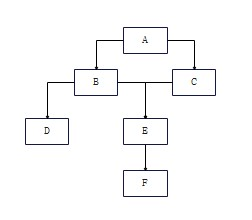
\includegraphics[width=0.5\linewidth]{CTG.jpg}
        \caption{控制流图}
        \label{fig:enter-label}
    \end{figure}
\end{description}

\subsubsection{确定支配集}

首先我们有:$\mathit{Dom}(n) = \{n\} \bigcup \left(\bigcap_{m\in \mathit{preds}(n)} \mathit{Dom}(m)\right)$。
即:一个节点的支配集等于其所有前驱节点(ctg)支配集的交集再并上自身。
这是显而易见的。根据支配集的定义,即所有必经节点的集合。根据定义,每个节点一定是自己的必经节点。所有前驱节点支配集的交集,即在表征所有前驱节点中共有的那些必经节点。因此,这两部分的并集就是这个节点的所有必经节点集合,也就是这个节点的支配集了。

我们可以通过对每个节点的迭代来计算支配集,即先假设所有节点的支配集都是节点全集,
并保证入口块没有入度(绝大多数情况下,入口块一定都没有入度),然后不断迭代直到收敛。
具体地,你可以在迭代的每一步都运行一遍 $\mathit{Dom}(n) \leftarrow \{n\} \bigcup
\left(\bigcap_{m\in \mathit{preds}(n)} \mathit{Dom}(m)\right)$,
直到一遍下来所有 $\mathit{Dom}(n)$ 不发生变化为止。
由于控制流图是前向传播的,所以这里迭代的顺序一般采用 BFS 序。

这样我们就获得了所有的 $\mathit{Dom}(n)$, 也就是获得了所有节点的支配关系。

\subsubsection{确定最近必经节点 (IDom)}

我们观察到支配集具有一个重要性质——节点 n 的支配集里任意两个不同的节点中,一个节点 A 必然是另一个节点 B 的必经节点。若非如此,就会存在只经过其中一个节点,就到达节点 n 的路径,这和支配集的性质相矛盾。因此,我们可以发现,每个节点支配集中的所有元素构成一条链,且直接支配节点的支配集元素比当前节点少1(实际上,如果按照这些元素的支配集元素个数排序,这些元素的支配集元素每个之间都差 1)。
因此,要确定当前节点的直接支配节点,只需要找到支配集元素个数为当前节点的支配集元素个数减 1 的节点。
注意,同样因为刚才的性质,这样的节点数量有且只有一个。

\subsubsection{支配树构建算法}

根据每个节点的直接支配节点,我们可以建构支配树。每个节点的直接支配节点到对应节点连边。
由于除入口节点外的每个节点入度都为 1,这样的图构成一棵支配树。


\subsubsection{确定支配边界}

根据支配边界的定义,一个节点 X 是节点 Y 的支配边界,当且仅当 Y 在 X 的一个控制流前驱节点的支配集中但 Y 不在 X 的支配集中。
因此,$n$ 是且仅是 $\bigcup_{m\in\mathit{preds}(n)}\left(\mathit{Dom}(m)-(\mathit{Dom}(n)-\{n\})\right)$
中元素的支配边界。

基于上面的原理,通过遍历所有基本块,我们就可以确定所有基本块的支配边界了。

\subsubsection{求支配集的其他方法}

以上的方法是通过迭代的方式求解支配集的。在控制流图节点数量较少的情况下,其时间复杂度是可以接受的。
然而,在某些极端的情况下,这种方法的时间复杂度是 $O(n^2)$ 的,可能会导致性能问题。以下给出两个求支配集的更高效的方法:

1. bitset 优化集合操作:注意到在迭代过程中,我们只需要对支配集进行交集、并集等操作,因此可以使用 bitset 位运算来加速这些操作。
2. Lengauer-Tarjan 算法:该算法可以在接近线性的时间复杂度内求解支配集。

以上两种做法,均在 OI-wiki \url{https://oi-wiki.org/graph/dominator-tree/} 中有详细介绍,感兴趣的读者可以参考。

\subsection{\texttt{phi} 指令放置算法}

\texttt{phi} 指令的放置分为两个步骤——预留 \texttt{phi} 指令和替换原来的变量使用。

对于加入 \texttt{phi} 指令,我们需要先收集所有被定义过的变量名(即 \texttt{alloca} 指令的结果),
再对每个变量名遍历找到所有变量的 def,在这些 def 所在块的支配边界的头部预留 \texttt{phi} 指令。
然后对预留了 \texttt{phi} 指令的块的支配边界头部再预留 \texttt{phi} 指令。重复操作,
直到没有新的支配边界或者对应块的支配边界已经预留了对应变量的 \texttt{phi} 指令。

\texttt{phi} 指令放置完毕后,我们需要对变量的使用进行重命名,即维护好之前提到的变量的 “版本”。
重命名的过程包括:为所有的 use 替换变量名、确定 \texttt{phi} 指令中不同块进入对应的值。一种可行的方式是为每个变量名开一个栈。这一步骤,我们可以在CFG上完成。具体的操作为
\begin{itemize}
  \item 在每个基本块中,首先应当对入口顶部的 \texttt{phi} 指令进行处理。我们要为这些\texttt{phi} 指令指定一个合适的\texttt{obj}名。然后,我们需要把这个\texttt{obj}名,压入这条\texttt{phi} 指令对应的 \texttt{alloca} 指令对应变量的对应栈中。对于每一个\texttt{alloca}指令对应的变量,我们都应该创建一个栈。栈顶就是当前的变量值。
  \item 在基本块中所有的操作都已经重写之后,我们将使用当前的形式名重写程序块在 CFG 中各后继节点中的适当 \texttt{phi} 指令的参数,即用当前对应栈的栈顶元素更新之。
  \item 最后,对当前基本块在支配树中的子节点进行递归处理,这是一个在支配树上 DFS 的过程。
  \item 当算法从一个基本块返回时,应当弹出所有的,在本基本块中压入的元素都应当被弹出。将所有的栈恢复原状。
\end{itemize}

请看下面的例子:

\begin{lstlisting}[language=LLVM]
define i32 @main() {
entry:
  %retval = alloca i32, align 4
  %x = alloca i32, align 4
  %y = alloca i32, align 4
  %b = alloca i32, align 4
  store i32 0, i32* %retval, align 4
  store i32 2, i32* %x, align 4
  store i32 3, i32* %y, align 4
  %0 = load i32, i32* %x, align 4
  %add = add nsw i32 %0, 1
  %1 = load i32, i32* %y, align 4
  %cmp = icmp sgt i32 %add, %1
  br i1 %cmp, label %if.then, label %if.else

if.then:                                          ; preds = %entry
  store i32 -1, i32* %b, align 4
  br label %if.end

if.else:                                          ; preds = %entry
  store i32 1, i32* %b, align 4
  br label %if.end

if.end:                                           ; preds = %if.else, %if.then
  %2 = load i32, i32* %b, align 4
  ret i32 %2
}
\end{lstlisting}

这个程序的支配树非常简单,即entry为根节点,剩余三个块均为entry的子节点。
经过\texttt{phi} 指令放置算法后, 我们的if.end块会变成这样:

\begin{lstlisting}[language=LLVM]
if.end:
  %b = phi i32 [ , %if.then ], [ , %if.else ]
  %2 = load i32, i32* %b, align 4
  ret i32 %2
\end{lstlisting}

为了方便演示,我们令这三个子节点的访问顺序是if.then, if.end, in.else.在访问完if.then块后,if.end块会变成:

\begin{lstlisting}[language=LLVM]
if.end:
  %b = phi i32 [ -1, %if.then ], [ , %if.else ]
  %2 = load i32, i32* %b, align 4
  ret i32 %2
\end{lstlisting}

在访问if.end块过程中,首先,重写\texttt{phi} 指令:

\begin{lstlisting}[language=LLVM]
; 不带优化的 LLVM IR
if.end:
  %phi = phi i32 [ -1, %if.then ], [ , %if.else ]
  %2 = load i32, i32* %b, align 4
  ret i32 %2
\end{lstlisting}

我们将\texttt{\%phi}这个名字压入\%b对应的栈中。 

检查该基本块,我们发现存在一条对\%b的\texttt{load} 指令。由于SSA的特性,Load的结果,即\%2的值从此被固定下来了。此时,\%b对应的栈,栈顶元素是\text{\%phi},我们可以另外在开一个map,存储\%2中的值是多少。经过改写,我们得到:

\begin{lstlisting}[language=LLVM]
if.end:
  %phi = phi i32 [ -1, %if.then ], [ , %if.else ]
  ret i32 %phi
\end{lstlisting}

然后,我们退出if.end块,同时将\%phi弹出。最后,我们访问if.else块,更新\texttt{phi}指令的值:

\begin{lstlisting}[language=LLVM]
if.end:
  %phi = phi i32 [ -1, %if.then ], [1, %if.else ]
  ret i32 %phi
\end{lstlisting}

大功告成!接下来要做的,就是诸如删除alloca指令之类的操作,这是很平凡的工作了。

\subsection{静态单赋值形式 (SSA) 的消除} \label{SSA-eliminate-phi}

经过 Mem2Reg,我们生成了很多 \texttt{phi}。然而,汇编中没有 \texttt{phi} 指令的直接对应,所以我们须将其消除,
用等价的其余指令如 \texttt{move} 来代替(注意这里的 \texttt{move} 属于内部实现,既不是 LLVM IR 的指令,
也不属于汇编)。一般地,我们在拥有 \texttt{phi} 指令的这个块的前驱块中插入一份拷贝,
例如图 \ref{fig:SSA-eliminate-phi-1}(BB 表示 \textbf{B}asic \textbf{B}lock)。

\begin{figure}[htb]
\centering
\begin{tikzpicture}[
squarednode/.style={rectangle, draw=black!100, fill=black!5, very thick, minimum size=5mm, align=center},
nothing/.style={circle, draw=white, minimum size=0}
]
\node[squarednode] (BB1) {BB1\\\texttt{x1=0}};
\node[nothing] (mid) [below=of BB1] {};
\node[squarednode] (BB2) [left=of mid] {BB2\\\texttt{x2=1}};
\node[squarednode] (BB3) [right=of mid] {BB3\\\texttt{x3=2}};
\node[squarednode] (BB4) [below=of mid] {BB4\\\texttt{x4=phi [x2, BB2], [x3, BB3]}};

\draw[thick,->] (BB1) -- (BB2.north);
\draw[thick,->] (BB1) -- (BB3.north);
\draw[thick,->] (BB2.south) -- (BB4);
\draw[thick,->] (BB3.south) -- (BB4);
\end{tikzpicture}
\begin{tikzpicture}[
squarednode/.style={rectangle, draw=black!100, fill=black!5, very thick, minimum size=5mm, align=center},
nothing/.style={circle, draw=white, minimum size=0}
]
\node[nothing] (BB1) {};
\node[nothing] (mid) [below=of BB1] {};
\node[nothing] (BB2) [left=of mid] {};
\node[nothing] (BB3) [right=of mid] {};
\node[nothing] (BB4) [below=of mid] {};

\draw[very thick, draw=black!50, ->] (BB2) -- (BB3);
\end{tikzpicture}
\begin{tikzpicture}[
squarednode/.style={rectangle, draw=black!100, fill=black!5, very thick, minimum size=5mm, align=center},
nothing/.style={circle, draw=white, minimum size=0}
]
\node[squarednode] (BB1) {BB1\\\texttt{x1=0}};
\node[nothing] (mid) [below=of BB1] {};
\node[squarednode] (BB2) [left=of mid] {BB2\\\texttt{x2=1}\\\texttt{x4=x2}};
\node[squarednode] (BB3) [right=of mid] {BB3\\\texttt{x3=2}\\\texttt{x4=x3}};
\node[squarednode] (BB4) [below=of mid] {BB4};

\draw[thick,->] (BB1) -- (BB2.north);
\draw[thick,->] (BB1) -- (BB3.north);
\draw[thick,->] (BB2.south) -- (BB4);
\draw[thick,->] (BB3.south) -- (BB4);
\end{tikzpicture}
\captionsetup{justification=centering}
\caption{左图为消除 \texttt{phi} 前的控制流图,右图为 \texttt{phi} 消除后的控制流图。\\可以发现右图将 \texttt{x4} 对应的取值插入到了 BB2 和 BB3 中。}
\label{fig:SSA-eliminate-phi-1}
\end{figure}

这样的操作能解决大部分的 \texttt{phi} 指令,但是还有一些特殊情况需要处理,例如图
\ref{fig:SSA-eliminate-phi-2} 的左图。

\begin{figure}[htb]
\centering
\begin{tikzpicture}[
squarednode/.style={rectangle, draw=black!100, fill=black!5, very thick, minimum size=5mm, align=center},
nothing/.style={circle, draw=white, minimum size=0}
]
\node[squarednode] (BB1) {BB1};
\node[nothing] (mid1) [right=of BB1] {};
\node[nothing] (mid2) [below=of BB1] {};
\node[squarednode] (BB2) [left=of mid2] {BB2};
\node[squarednode] (BB3) [right=of mid2] {BB3};
\node[squarednode] (BB4) [right=of mid1] {BB4};

\draw[thick,->] (BB1) -- (BB2);
\draw[thick,->] (BB1) -- (BB3);
\draw[thick,->] (BB4.south) -- (BB3);
\end{tikzpicture}
\begin{tikzpicture}[
squarednode/.style={rectangle, draw=black!100, fill=black!5, very thick, minimum size=5mm, align=center},
nothing/.style={circle, draw=white, minimum size=0}
]
\node[nothing] (BB1) {};
\node[nothing] (mid) [below=of BB1] {};
\node[nothing] (BB2) [left=of mid] {};
\node[nothing] (BB3) [right=of mid] {};
\node[nothing] (BB4) [below=of mid] {};

\draw[very thick, draw=black!50, ->] (BB2) -- (BB3);
\end{tikzpicture}
\begin{tikzpicture}[
squarednode/.style={rectangle, draw=black!100, fill=black!5, very thick, minimum size=5mm, align=center},
nothing/.style={circle, draw=white, minimum size=0}
]
\node[squarednode] (BB1) {BB1};
\node[nothing] (mid1) [below=of BB1] {};
\node[squarednode] (BB2) [left=of mid1] {BB2};
\node[squarednode] (BB5) [right=of mid1] {BB5};
\node[nothing] (mid2) [right=of BB5] {};
\node[squarednode] (BB4) [right=of mid2] {BB4};
\node[squarednode] (BB3) [below=of mid2] {BB3};

\draw[thick,->] (BB1) -- (BB2);
\draw[thick,->] (BB1) -- (BB5);
\draw[thick,->] (BB5) -- (BB3);
\draw[thick,->] (BB4.south) -- (BB3);
\end{tikzpicture}
\captionsetup{justification=centering}
\caption{左图为原控制流图,右图为插入新基本块 BB5 后的控制流图。\\BB1 到 BB3 构成 critical edge,有数据冲突隐患,因此二者间需要插入空基本块 BB5 以消除 critical edge。}
\label{fig:SSA-eliminate-phi-2}
\end{figure}

我们看到图 \ref{fig:SSA-eliminate-phi-2} 左图的 BB1 有两个后继,BB3 有两个前驱。
假设 BB2、BB3 都有 \texttt{phi} 指令,则它们都会往 BB1 插入拷贝,这就会导致该变量在 BB1 上被修改,
从而影响到 BB2 所在的分支进而引起数据冲突。我们发现,BB1 与 BB3 之间的这条边有这样的特点:
出端有多个后继且入端有多个前驱。我们称这样的边为 \textbf{critical edge}。

所有的 critical edge 都可能会引起上述的数据冲突。
为了解决 critical edge,我们需要在 critical edge 中间插入一个新的空基本块 BB5 以消除 critical edge。
BB3 中的 \texttt{phi} 指令会往 BB5 和 BB4 中插入拷贝,而 BB2 中的 \texttt{phi} 指令会往
BB1 中插入拷贝,这样就不会有数据冲突了。

值得一提的是,在上图中,BB2 和 BB1 之间的 edge 也是 critical edge(BB2 既然有
\texttt{phi} 指令,它必定是有多个前驱的,否则这个 \texttt{phi} 指令可以直接被消除)。
为了方便展示,图里并没有画出来,实际上也需要在此插上空块。

同时,在汇编代码翻译的过程中,我们也需要注意数据冲突发生的可能性。比如说,我们可能在翻译过程中,产生这样的语句:
\begin{lstlisting}
	mv	a2, a0
	mv	a1, a2
 	mv	a0, a1
\end{lstlisting}

经过如上精彩绝伦的操作,我们成功地把三个寄存器都赋成了原先a0的值,但这大抵不是我们所希望的。在这个过程中,我们可以引入一些临时变量,或者合理地安排各变量之间的顺序来解决这个问题。

\section{寄存器分配:冲突图与图染色算法}

寄存器分配的目标有二:
\begin{itemize}
    \item 尽可能地将变量(尤其是临时变量)分配到寄存器中,而不是内存中。
    \item 尽量为 \texttt{move} 指令(由静态单赋值形式的消除而产生,见 \ref{SSA-eliminate-phi})
        的 source 和 destination 分配同一个寄存器。
\end{itemize}
前者是为了减少内存读写占用的时间,因而希望尽可能将变量分配到寄存器中,使其在使用时无需访存;后者是为了减少使用的寄存器,同时减少无用指令,因而基于 \texttt{move} 指令的需求,希望提升 \texttt{phi} 指令的运行效率。

为了方便设计分配算法,我们将寄存器分配抽象为图染色问题:
\begin{itemize}
    \item 将变量抽象为点;
    \item 将分配寄存器抽象为染色。如果能够染色,表明对应的变量在其生命周期里可以一直保存在寄存器中。
    \item 如果两个变量不能保存在同一个寄存器里(存在 “冲突”),那么这二者之间连边。规定染色时连边的两点不能同色。
        存在冲突意味着两个变量同时活跃。注意冲突是相互的,所以这里的边是无向边。
    \item 由于寄存器的数量是有限的,因此有可能会发生一个图无法被染色。在这种情况下,为了提升性能,
        我们希望将更少的变量存到内存(栈)中并再对剩下的图进行染色。把变量存在栈上,
        就意味着它不需要使用任何寄存器资源,即我们可以将它从这张图中删除。这个过程被称为\textbf{溢出 (spill)}。
\end{itemize}

由于上面所述的图表示了冲突关系,因此被称作冲突图 (Interference Graph)。

注意,判断一个图是否能被 K-染色是一个 NP 难问题,因此不存在一个多项式时间算法来给出染色方案。
因此我们不能在多项式时间内找到最优算法,所以我们这里的染色算法是启发式的。

本部分中,我们将以《现代编译原理》\cite{TigerBook}中的算法为例,介绍其中一系列的处理阶段,
然后展示寄存器分配的流程(章节 \ref{opt-graph-workflow})。关于具体的代码实现,强烈建议参考原书,
原书提供了详细的解释和伪代码实现。

\subsection{建图 (Build)} \label{opt-graph-build}

我们需要先构建冲突图。最基础的冲突关系是两个变量同时活跃。

通过基本块的活跃信息,以及活跃分析的数据流方程(公式 \ref{live-analysis-data-flow-1},
\ref{live-analysis-data-flow-2}, \ref{live-analysis-data-flow-3}),
我们可以获得每条指令的入口活跃和出口活跃变量。

我们注意到,对于每一个 def,其与所有入口活跃的变量冲突。因此,我们只需要顺序遍历块中指令,
对所有 def 向此时存活的其它变量连边,表示它的生命周期的开始与其他存活的变量的生命周期有重合。

\subsection{简化 (Simplify)} \label{opt-graph-simplify}

我们观察到,对于一张图,假设我们现在想用 K 种颜色来染色,则对于图中所有度数小于 K 的节点,
无论其余的点采取何种染色方案,它都可以找到至少一种颜色可以染。那么我们可以先不染这种点。
也就是说,我们把这样的点以及其连着的边从冲突图上去掉,
然后染好剩下的图,再逆向地按照删点顺序把这些点染上颜色,就能构造出一种染色方案。
具体来说,我们可以把这样的节点丢进一个栈(我们用 \texttt{selectStack} 来表示这个栈),
代表我们将要在染色时对这里面的节点进行这一轮的染色。在后面的内容中,我们将度数小于 K 的节点称为低度数节点,
将度数不小于 K 的节点称为高度数节点。

下面会提到,传送有关 (move related) 的节点具有合并的可能性,故而在这一步,我们不对其进行简化。
一个节点是传送有关的当且仅当它是 \texttt{move} 指令的一个操作数(src 或 dest),否则它是传送无关的。
简化过程只处理传送无关的节点。

而在简化过程中某一时刻,这张图可能只包含度数大于等于 K 的节点和传送有关的节点,这时我们的简化算法就无法继续进行了。
这时我们需要选择一个节点,但我们对这个节点的溢出做出乐观的估计,即我们希望这个节点在最后是可以被染色的。
因此我们把这个被选中的节点删除并压入 \texttt{selectStack} 中,继续我们的简化处理。

\subsection{合并 (Coalesce)} \label{opt-graph-coalesce}

两个变量可以(在冲突图上)合并当且仅当它们之间无边并且它们由一个 \texttt{move} 指令相连(src 和 dest)。
通过对冲突图的分析,我们很容易能减少冗余的传送指令。合并指的是两个节点合并成一个节点,
其邻节点为这两个节点原来邻居节点的并集。容易想到,合并这一过程,我们可以用并查集来进行维护。
但要注意的是,并不是只要符合定义都可以直接合并,因为合并完之后图可能从可 K-着色的变为不可 K-着色的,从而造成溢出,这样并不优。具体地,合并时可以参考这两条规则:
\begin{itemize}
    \item Briggs 规则:合并后产生的节点所拥有的度数不小于 K 的邻节点个数小于 K。
        这样的节点在简化后会将这个合并后的节点移走。
    \item George 规则:a 和 b 可以合并的条件是:对 a 的每一个邻居 t,t 的度数小于 K 或者 t 与 b 冲突。
        这保证了合并这两个节点不会让染色问题更难解决。
\end{itemize}

你可以在两条规则都满足的前提下才进行合并,当然你也可以只满足其中一条,或者加入一些对节点的特判,等等。
这两条规则都是安全的,即当通过任意一条规则合并成功时,这张图不会从可 K-着色的变成不可 K-着色的。
当合并发生之后,新产生的节点将不再是传送有关的节点,因此我们可以将其放入待简化的工作表中,使得简化过程能进一步进行下去。

\subsection{冻结 (Freeze)} \label{opt-graph-freeze}

前面提到合并有条件。在建图后维护所有工作表的时候,传送有关的节点因为有合并的希望暂时不放入待简化的工作表中。
如果传送与合并都无法进行,我们选择一个低度数的传送有关的节点,冻结与其有关的所有传送,即放弃这些传送的合并,
使得其在下一轮被简化。

\subsection{选择溢出变量 (Select Spill)} \label{opt-graph-select-spill}

我们用 \texttt{spillWorklist} 表示被筛选出来的度数大于 K 的节点的集合。
选择 \texttt{spillWorklist} 中的一个高度数节点进行溢出。
至于如何选择这一节点,你有很多种估价方式,比如选择度数最大的,或者选择活跃区间最长的,
或者选择度数和活跃区间长度的乘积最大的,等等。
溢出的节点,我们扔进另一个栈(用 \texttt{spilledStack} 表示)中,等待分配栈空间给这些变量。

溢出的节点加入简化工作表等待被删除(虽然它并非低度数节点),等到染色时会区分可染色节点和溢出节点。

\subsection{进行染色 (Assign Color)} \label{opt-graph-assign-color}

对 \texttt{selectStack}(本轮需要染色的节点)里的点进行染色。
我们从一个空的图开始,通过重复地将栈顶节点添加到图中来重建冲突图。
根据简化阶段的性质,我们可以保证每次添加的节点都会有一种它能使用的颜色。
如果颜色不够,把当前节点放到已溢出表 \texttt{spilledStack} 中。

\subsection{相关代码重写 (Rewrite)} \label{opt-graph-rewrite}

如果存在溢出,我们需要逐个为其分配存储单元(一般来说是分配栈上的空间)。
然后给这些变量插入对应的 load 和 store。def 后插 store,use 前插 load。
我们就把这一溢出的变量变成了许多新创建的小临时变量(生命周期短),
因此我们需要对改变后的图重新调用一次整个过程。

\subsection{预着色节点的处理}

有一些临时变量需要被放在给定的寄存器上,比如函数的参数、返回地址等等,这些变量不能随意地分配颜色。
我们称这些变量是\textbf{预着色 (precolored)} 的。
在建图的时候,我们需要把这些变量加入冲突图,但是不能把它们加入工作表中,即它们不能被简化,更不可能被溢出。

因此我们可以默认这些节点的度数为无穷大,这样它们就不会被简化。这样一来我们在简化步骤中只要简化到只剩预着色节点、传送有关节点和高度数节点的图就可以了。
这一般不会引起问题,因为这些预着色的变量通常有着很短的生命周期。

\subsection{图染色流程} \label{opt-graph-workflow}

\begin{remark}
我们这里不会介绍具体的逻辑。如果需要了解具体的代码逻辑,请参考《现代编译原理》\cite{TigerBook}。
\end{remark}

图染色的流程如下:
\begin{enumerate}
  \item 进行活跃分析。

  \item 建立冲突图(章节 \ref{opt-graph-build})。

  \item 初始化每个阶段待处理的变量列表。
    \begin{itemize}
      \item 简化阶段(章节 \ref{opt-graph-simplify}):所有度数小于 K 且不包含 \texttt{move} 的节点。
      \item 合并阶段(章节 \ref{opt-graph-coalesce}):所有 \texttt{move} 的指令。
      \item 冻结阶段(章节 \ref{opt-graph-freeze}):所有度数小于 K 且与 \texttt{move} 相关的点。
      \item 选择溢出变量过程(章节 \ref{opt-graph-select-spill}):所有度数不小于 K 的节点。
    \end{itemize}

  \item 执行以下部分直到所有阶段都没有待处理的变量:(注意,每次执行时从上至下选取第一个列表非空的阶段处理)
    \begin{enumerate}
      \item 简化阶段(章节 \ref{opt-graph-simplify})
      \item 合并阶段(章节 \ref{opt-graph-coalesce})
      \item 冻结阶段(章节 \ref{opt-graph-freeze})
      \item 选择溢出变量过程(章节 \ref{opt-graph-select-spill})
    \end{enumerate}

  \item 进行染色(章节 \ref{opt-graph-assign-color})。

  \item 如果存在溢出的变量,则重写相关代码(章节 \ref{opt-graph-rewrite}),注意重写完需要再次进行图染色。
\end{enumerate}

\section{寄存器分配:线性扫描算法}
当你读完上面的图染色算法之后,有没有感到一头雾水,有没有感到无所适从?诚然,图染色算法分配寄存器的质量比较高,但是该算法时间复杂度较高,同时代码本身也较为复杂。为此,在这里谨介绍另外一种常见的寄存器分配算法:线性扫描算法。这种算法的时间复杂度理论上来说是线性的,同时编码较为简单。尽管其寄存器分配的质量较图染色算法稍差一些,但最坏情况下,质量下降不会超过10\%。目前,llvm中的basic寄存器分配策略,和greedy寄存器分配策略,基本是在线性扫描算法的基础上改进得来的。

线性扫描算法的思路是非常符合直觉的。首先,我们确定每条语句的线性序。说人话,就是给每条语句指派一个唯一的编号,使得每条语句之间的编号都有严格的大小关系。然后,我们通过活跃分析算法,计算得到每个变量的“活跃区间”:即该变量仅在编号为$[a, b]$的语句中活跃。这个区间越精确越好。然后,我们将这些区间按照左端点的大小进行排序,从而构建一优先级队列,队头为左端点最少的一元素。最后,我们不断对该优先级队列执行出队操作。并且检查当前是否有寄存器空闲,并尝试分配之。否则,则将其溢出至栈上。

\subsection{确定语句线性序}
    \begin{figure}[h]
        \centering
        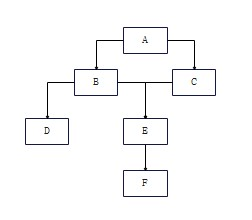
\includegraphics[width=0.5\linewidth]{CTG.jpg}
        \caption{控制流图}
        \label{fig:enter-label}
    \end{figure}
我们再以这张控制流图为例,来介绍确定语句线性序的算法。根据论文中的做法,我们从CTG的入口开始执行DFS,将每个结点都访问一次,在\textbf{退出}某一个节点时,输出该变量。那么,我们可以轻易得到这样的dfs顺序:$A\to B, B\to D, B\to E, E\to F, A\to C$,得到的输出结果是$D, F, E, B, C, A$。
然后,我们将其逆过来,即得到各基本块之间的线性序,即$A, C, B, E, F, D$。这就是基本块之间的线性序关系了。接下来,我们要做的无非是在基本块内对每一句语句进行标号了。这是平凡的。

\subsection{确定活跃区间}
这一部分请见活跃分析章节。我们只需要记录下每条语句处的活跃变量,根据每条语句的标号,对应地去更新这些变量的活跃变量即可。

\subsection{活跃区间排序}
\sout{不会吧不会吧,不会还有人优先级队列也不会用吧?真是杂鱼呢$\sim$}
这一部分的工作是非常平凡的。我们可以创造一个区间类,挑选一个心仪的容器,重载比较运算符,或者是用仿函数的方式确定区间类之间的大小关系进行排序即可。

\subsection{寄存器分配}
正如在该部分总述中的做法,不断对优先级队列执行出队操作,并检查是否有寄存器空闲:即该寄存器从来没有被指派过变量,或者指派给该寄存器之变量的活跃区间右端点小于当前分配变量的活跃区间之左端点。若有,则将当前变量分配给空闲的寄存器。如果没有,则将其溢出至栈上。

\subsection{总结}
不难发现,线性扫描算法是一种非常简洁,明确的寄存器分配算法。此外,如果向对线性扫描算法执行一定的优化,可以考虑进行区间拆分等操作,或是探索更合适的线性排序方法,或者可以考虑如何更好地对活跃区间排序等,于此不复赘述。

让我们动手吧!

\section{SCCP: Sparse Conditional Constant Propagation 常量传播}

在真实的 C 语言程序中,由于宏展开或函数内联优化,可能会生成如下类似的代码:

\begin{lstlisting}[language=LLVM]
.bb1:								; # entry
    %add-0 = add i32 1, 2
    %mul-0 = mul i32 %add-0, 10
    %sub-0 = sub i32 %mul-0, 100
    %cmp-0 = icmp slt i32 %sub-0, 100
    br i1 %cmp-0, label %.bb3, label %.bb4
.bb3:								; # branch body
    br label %.bb2
.bb4:								; # branch fail
    br label %.bb2
.bb2:								; # branch exit
    %x-0 = phi i32 [ 200 , %.bb4 ], [ 100 , %.bb3 ]
    ret i32 %x-0
\end{lstlisting}

通过观察可以发现,该函数最终一定返回 100,因为涉及的计算全是常量,分支条件也是常量。一个自然的问题是:如何系统性地识别程序中的所有常量?

在论文 \textit{Constant Propagation with Conditional Branches}\cite{SCCP} 中,作者提出了一种尽可能识别并传播常量的方法。
由于该方法基于 SSA 形式(静态单赋值形式),它的时间复杂度是线性的,因此被称为稀疏(Sparse)。

\subsection{基础 —— SCP}

首先,我们讨论不含条件分支的稀疏常量传播(Sparse Constant Propagation, SCP)。通过迭代的方式逐步确定程序中的常量。

初始时,我们假设所有值都有可能成为常量,并为每个表达式的结果标记为“未定义”。接着从入口块开始,依次遍历表达式。
对于纯函数表达式(没有外部状态依赖的表达式,如算术运算、比较以及无副作用的函数),
如果所有操作数都是常量或通过某些规则可确定结果(如 $0$ 乘任何数都为 $0$),
则更新表达式结果为“常量”。如果先前标记为“常量”的结果发生变化,则更新为“非常量”。若无法确定结果,则直接标记为“非常量”。

需要特别注意的是,$\phi$ 函数仅当所有入口块传入的值都是相同的常量时,才会被标记为“常量”。

每次更新表达式的标记后,我们都会更新使用该表达式的所有地方。由于程序是基于 SSA 形式的,因此我们可以沿着 def-use 链传播变化。
该过程中的每个表达式最多遍历 $3 * (\text{操作数} + 1)$ 次,因为状态转换只可能是“未定义 -> 常量 -> 非常量”。
因此,SCP 算法的时间复杂度是线性的。在算法结束后,所有被标记为常量的表达式都将被替换为对应的常量。

\subsection{改进 —— SCCP}

注意到以上 SCP 算法对于分支是无能为力的,必须遍历所有可能的分支。而对于 \text{\%phi} 函数,我们要求所有的入口都是相同的常量,
这显然过于苛刻。事实上,在我们给出的例子里面,由于只有一个分支可达,所以这个 \text{\%phi} 函数的结果是可以确定的。

一个暴力的解决方案是,在跑完 SCP 后,我们对于所有条件为常量的的分支语句特判,转化为跳转指令。在全部替换结束后,
再把所有由入口块不可到达的块删除,并且删除由这些块引出的 \text{\%phi} 函数。

(笔者注:这其实可以是单独的一个优化步骤,把所有不可达的分支删除,并且简化控制流图。
常用于某些未定义行为的优化。编译器总是假定程序是没有未定义行为的,因此如果一个分支有未定义行为,我们可以假定这个分支是不可达的。
同时,一个函数必须要有返回语句 (void 类型也有 ret void),否则也是未定义行为。
因此,我们可以分别从入口块和返回块开始,分别正向和反向遍历,标记所有可达的块。
只有那些可以从入口块到达的块,以及可以到达返回块的块,才被保留。其他的块都将会被删除。请注意,在删除块的时候,需要检查其后继块,
删除对应的 \text{\%phi} 函数的对应入口。)

当然,该方法在最坏情况下需要额外执行分支数量的次数。我们可以通过改进 SCP 算法来减少这个数量。我们可以在 SCP 算法中加入对分支的处理,
即为 Sparse Conditional Constant Propagation (SCCP)。

首先,我们需要维护两个队列:一个是表达式队列,另一个是控制流边队列。一个小 trick 是加入一个虚拟块作为入口点的前驱块,
初始化控制流队列为从虚拟块到入口块的边,而表达式队列最初为空。

在每一轮迭代中,我们尝试从两个dui'lie中取出一个元素。如果是控制流队列的元素(即一条边,从块 $A$ 到 $B$),
我们首先标记 $B$ 从 $A$ 来过。如果之前 $B$ 从 $A$ 来过,那么直接跳过本次操作。否则,我们会遍历 $B$ 块的所有
\text{\%phi} 函数,以及控制流语句,按照新的规则更新 (见下文)。特别地,如果在此之前块 $B$ 从没有被访问过 (即第一次访问),
那么我们需要把 $B$ 中的其他语句也顺序访问一遍,以确保我们不会遗漏任何一个表达式。所以单个块内的遍历顺序是:
\text{\%phi} 函数 -> (如果是第一次,其他语句) -> 控制流语句。

如果是表达式队列的元素,我们基本按照 SCP 的规则更新,但是细节上有所不同。
对于 \text{\%phi} 函数,我们只需检查其当前所有的来过的入口的值是否都是常量,以此来更新。
比如块 $C$ 当前仅仅从 $A$ 和 $B$ 来过,那么只需检查每个 \text{\%phi} 函数的来自 $A$ 和 $B$ 的值是否相同即可。
对于无条件跳转 \text{br} 语句,我们需要把 “当前块” 到 “跳往块” 的边加入控制流队列。对于条件跳转 \text{br} 语句,
如果条件被标记为 “未定义”,则不操作。如果被标记为 “常量”,则根据条件跳转的结果,
把 “当前块” 到 “跳往块” 的那条边加入控制流队列。否则,需要将两条边都加入控制流队列。
特别地,当一个表达式的标记更新的时候,我们需要把所有使用这个表达式的地方加入表达式队列。

\printbibliography[heading=bibintoc, title=\ebibname]
\appendix

\chapter{致谢}

\end{document}
